%%%%%%%%%%%%%%%%%%%%%%%%%%%%%%%%%%%%%%%%%%%%%%%%%%%%%%%%%%%%%%%%%%%%%%%%%%%%%%%
%                                                                             %
% VARIATIONAL MONTE CARLO METHODS FOR QUANTUM DOTS, by Matteo Seclì           %
%                                                                             %
% This eBook is meant to be used as the BSc Thesis of the author.             %
% The predicted date of the discussion is 22/07/2015 at the University of     %
% Trento.                                                                     %
%                                                                             %
% For licensing information, look at the LICENSE file shipped with this       %
% document.                                                                   %
%                                                                             %
% The original location of this project is at                                 %
% https://github.com/matteosecli/QMC.                                         %
%                                                                             %
% Title: Variational Monte Carlo Methods for quantum dots                     %
%                                                                             %
% Author: Matteo Seclì <secli.matteo@gmail.com>                               %
%                                                                             %
% Language: English                                                           %
%                                                                             %
% Character set encoding: UTF-8                                               %
%                                                                             %
% *** START OF THIS BACHELOR THESIS PROJECT ***                               %
%                                                                             %
%%%%%%%%%%%%%%%%%%%%%%%%%%%%%%%%%%%%%%%%%%%%%%%%%%%%%%%%%%%%%%%%%%%%%%%%%%%%%%%


%%%%%%%%%%%%%%%%%%%%%%%%%%%%%%%%%%%%%%%%%%%%%%%%%%%%%%%%%%%
% Basic class definitions, typesetting, bibliography      %
%%%%%%%%%%%%%%%%%%%%%%%%%%%%%%%%%%%%%%%%%%%%%%%%%%%%%%%%%%%
\documentclass[a4paper,twoside,11pt]{book}
\usepackage[utf8]{inputenc}
\usepackage{type1cm}
\usepackage{setspace}
\usepackage[english]{babel}
\usepackage{datetime}

\usepackage[backend=bibtex, sorting=none]{biblatex}
\addbibresource{bibliography.bib}
%%%%%%%%%%%%%%%%%%%%%%%%%%%%%%%%%%%%%%%%%%%%%%%%%%%%%%%%%%%
% Hyperref configuration                                  %
%%%%%%%%%%%%%%%%%%%%%%%%%%%%%%%%%%%%%%%%%%%%%%%%%%%%%%%%%%%
\usepackage[%hypertex,
	unicode=true,
	plainpages = false, 
	pdfpagelabels, 
	bookmarks=true,
	bookmarksnumbered=true,
    bookmarksopen=true,
	breaklinks=true,
	backref=false,
	colorlinks=true,
	linkcolor = blue,		% Use "blue" if you want to highlight them
	urlcolor  = blue,
	citecolor = red,
	anchorcolor = green,
	hyperindex = true,
	linktocpage = true,
	hyperfigures
]{hyperref}


%%%%%%%%%%%%%%%%%%%%%%%%%%%%%%%%%%%%%%%%%%%%%%%%%%%%%%%%%%%
% Grahpics                                                %
%%%%%%%%%%%%%%%%%%%%%%%%%%%%%%%%%%%%%%%%%%%%%%%%%%%%%%%%%%%
\usepackage{blochsphere}


\usepackage{graphicx}
\usepackage{xcolor}
\graphicspath{{figures/PNG/}{figures/PDF/}{figures/}}
\usepackage{tikz}
\usepackage[siunitx]{circuitikz}


%%%%%%%%%%%%%%%%%%%%%%%%%%%%%%%%%%%%%%%%%%%%%%%%%%%%%%%%%%%
% Standard environments                                   %
%%%%%%%%%%%%%%%%%%%%%%%%%%%%%%%%%%%%%%%%%%%%%%%%%%%%%%%%%%%
\usepackage{float}
\usepackage[font={small,it}]{caption}[2013/01/06] % Minimum version required for incompatibility with breqn
\usepackage{subcaption}
\usepackage{listingsutf8}
\usepackage{enumitem}
\usepackage{amsmath,scalerel}

\DeclareMathOperator*{\Bigcdot}{\scalerel*{\cdot}{\bigodot}}

%%%%%%%%%%%%%%%%%%%%%%%%%%%%%%%%%%%%%%%%%%%%%%%%%%%%%%%%%%%
% Math                                                    %
%%%%%%%%%%%%%%%%%%%%%%%%%%%%%%%%%%%%%%%%%%%%%%%%%%%%%%%%%%%
\usepackage{amsmath}
\usepackage{amssymb}	
\usepackage{float}
\usepackage{amsthm}
\usepackage{cancel}
\usepackage{braket}
\usepackage{siunitx}
\DeclareSIUnit\atomicunit{a.u.}
\usepackage{breqn}
\usepackage{geometry}
\usepackage{tikz}
\usepackage{wrapfig}
\usetikzlibrary{quantikz}
\usepackage{braket}
\renewenvironment{proof}{\vskip 1em \noindent\textsc{Proof:}}{\begin{flushright}$\blacksquare$\end{flushright}\vskip 1em}
\usepackage{mathtools}
\DeclarePairedDelimiter\ceil{\lceil}{\rceil}
\DeclarePairedDelimiter\floor{\lfloor}{\rfloor}

%%%%%%%%%%%%%%%%%%%%%%%%%%%%%%%%%%%%%%%%%%%%%%%%%%%%%%%%%%%
% datetime specific configuration                         %
%%%%%%%%%%%%%%%%%%%%%%%%%%%%%%%%%%%%%%%%%%%%%%%%%%%%%%%%%%%
\newdateformat{monthyear}{\monthname[\THEMONTH] \THEYEAR}


%%%%%%%%%%%%%%%%%%%%%%%%%%%%%%%%%%%%%%%%%%%%%%%%%%%%%%%%%%%
% TikZ specific configuration                             %
%%%%%%%%%%%%%%%%%%%%%%%%%%%%%%%%%%%%%%%%%%%%%%%%%%%%%%%%%%%
\usetikzlibrary{shapes.geometric, arrows, patterns}
\tikzstyle{startstop} = [rectangle, rounded corners, minimum width=3cm, minimum height=1cm,text centered, draw=black, fill=red!30]
\tikzstyle{io} = [trapezium, trapezium left angle=70, trapezium right angle=110, minimum width=3cm, minimum height=1cm, text centered, draw=black, fill=blue!30]
\tikzstyle{process} = [rectangle, minimum width=3cm, minimum height=1cm, text centered, text width=3cm, draw=black, fill=orange!30]
\tikzstyle{decision} = [diamond, minimum width=3cm, minimum height=1cm, text centered, draw=black, fill=green!30]
\tikzstyle{arrow} = [thick,->,>=stealth]


%%%%%%%%%%%%%%%%%%%%%%%%%%%%%%%%%%%%%%%%%%%%%%%%%%%%%%%%%%%
% xcolor specific configuration                           %
%%%%%%%%%%%%%%%%%%%%%%%%%%%%%%%%%%%%%%%%%%%%%%%%%%%%%%%%%%%
\definecolor{dkgreen}{rgb}{0,0.6,0}
\definecolor{dred}{rgb}{0.545,0,0}
\definecolor{dblue}{rgb}{0,0,0.545}
\definecolor{lgrey}{rgb}{0.9,0.9,0.9}
\definecolor{gray}{rgb}{0.4,0.4,0.4}
\definecolor{darkblue}{rgb}{0.0,0.0,0.6}


%%%%%%%%%%%%%%%%%%%%%%%%%%%%%%%%%%%%%%%%%%%%%%%%%%%%%%%%%%%
% ListingsUTF8 specific configuration                     %
%%%%%%%%%%%%%%%%%%%%%%%%%%%%%%%%%%%%%%%%%%%%%%%%%%%%%%%%%%%
\lstdefinelanguage{cpp}{
	backgroundcolor=\color{lgrey},  
	basicstyle=\footnotesize \ttfamily \color{black} \bfseries,   
	breakatwhitespace=false,       
	breaklines=true,               
	captionpos=b,                   
	commentstyle=\color{dkgreen},   
	deletekeywords={...},          
	escapeinside={\%*}{*)},                  
	frame=single,                  
	language=C++,                
	keywordstyle=\color{purple},  
	morekeywords={BRIEFDescriptorConfig,string,TiXmlNode,DetectorDescriptorConfigContainer,
		istringstream,cerr,exit}, 
	identifierstyle=\color{black},
	stringstyle=\color{blue},      
	numbers=right,                 
	numbersep=5pt,                  
	numberstyle=\tiny\color{black}, 
	rulecolor=\color{black},        
	showspaces=false,               
	showstringspaces=false,        
	showtabs=false,                
	stepnumber=1,                   
	tabsize=5,                     
	title=\lstname,                 
}


%%%%%%%%%%%%%%%%%%%%%%%%%%%%%%%%%%%%%%%%%%%%%%%%%%%%%%%%%%%
% Some black magic                                        %
%%%%%%%%%%%%%%%%%%%%%%%%%%%%%%%%%%%%%%%%%%%%%%%%%%%%%%%%%%%
%\makeatletter
%	\renewcommand{\bibsection}{\chapter{\bibname}}
%\makeatother


%%%%%%%%%%%%%%%%%%%%%%%%%%%%%%%%%%%%%%%%%%%%%%%%%%%%%%%%%%%
% Metadata                                                %
%%%%%%%%%%%%%%%%%%%%%%%%%%%%%%%%%%%%%%%%%%%%%%%%%%%%%%%%%%%
\def\THauthor{Alexander Ferraro}
\def\THsupervisor{Philipp Hans Juergen Hauke, University of Trento}
%\def\THextrasupervisor{Francesco Pederiva, UniTN}
\def\THtitle{Quantum Error Correction} % title
\def\THdate{\monthyear\today}
\def\THplace{Trento}
\title{\THtitle}
\author{\THauthor}


%%%%%%%%%%%%%%%%%%%%%%%%%%%%%%%%%%%%%%%%%%%%%%%%%%%%%%%%%%%
% Actual text                                             %
%%%%%%%%%%%%%%%%%%%%%%%%%%%%%%%%%%%%%%%%%%%%%%%%%%%%%%%%%%%
\newtheorem{theorem}{Theorem}
\newtheorem{definition}{Definition}[chapter]
\begin{document}

\frontmatter
%%%%%%%%%%%%%%%%%%%%%%%%%%%%%%%%%%%%%%%%%%%%%%%%%%%%%%%%%%%
%                                                         %
% TITLEPAGE                                               %
%                                                         %
%                                                         %
% This file is part of a BSc Thesis Project. See the      %
% LICENSE file for more information about licensing.      %
%                                                         %
% Author:     Matteo Seclì <secli.matteo@gmail.com>       %
% A.Y.:       2014/2015                                   %
% URL:        https://github.com/matteosecli/QMC          %
%                                                         %
%%%%%%%%%%%%%%%%%%%%%%%%%%%%%%%%%%%%%%%%%%%%%%%%%%%%%%%%%%%

\graphicspath{{Frontmatter/figures/PNG/}{Frontmatter/figures/PDF/}{Frontmatter/figures/}}

\begin{titlepage}
	\newgeometry{margin=3.5cm}
	
	\begin{center}
	
		% Logo
		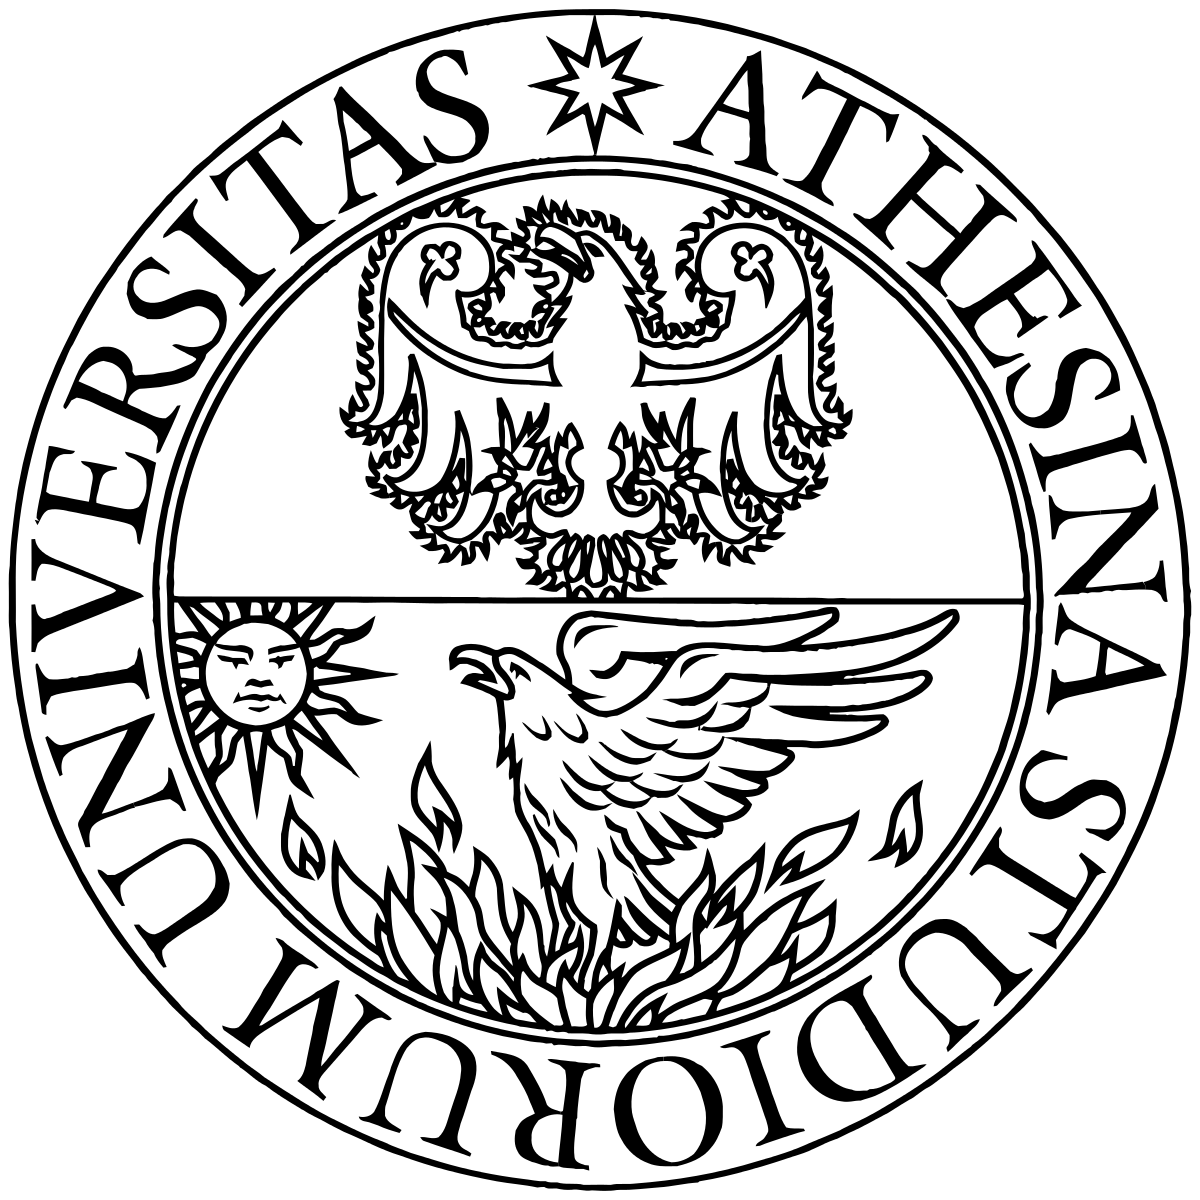
\includegraphics[scale=0.12]{logo_unitn}\\[0.4cm]
			
		\vspace{0.8cm}
		
		{ \Huge \scshape University of Trento }\\[0.25cm]
		{ \Large \scshape Department of Physics }\\[2cm]

		{ \Large \scshape Thesis }\\[0.05cm]
		{ \itshape for the degree in }\\[0.05cm]
		{ \Large \scshape Bachelor of Science }\\[2cm]
		
		
		% Title
		{ \huge \bfseries \THtitle }
		
		\vfill
				
		% Author and supervisor
		\begin{minipage}[t]{0.45\textwidth}
			\begin{flushleft} %\large
				{ \large \scshape Supervisor: } \\[0.25cm]
				{ Prof. \THsupervisor }\\[0.10cm]
			\end{flushleft}
		\end{minipage}
		\begin{minipage}[t]{0.45\textwidth}
			\begin{flushright} %\large
				{ \large \scshape Candidate: }\\[0.25cm]
				{ \THauthor }
			\end{flushright}
		\end{minipage}
		
		\vspace{2cm}
		
		% Bottom of the page
		{\large \scshape Academic Year 2020/2021}
		
	\end{center}
	
	\restoregeometry
\end{titlepage}
\onehalfspacing	% Set 1.5 lines spacing for better readability
%%%%%%%%%%%%%%%%%%%%%%%%%%%%%%%%%%%%%%%%%%%%%%%%%%%%%%%%%%%
%                                                         %
% PREFACE                                                 %
%                                                         %
% This file is part of a BSc Thesis Project. See the      %
% LICENSE file for more information about licensing.      %
%                                                         %
% Author:     Matteo Seclì <secli.matteo@gmail.com>       %
% A.Y.:       2014/2015                                   %
% URL:        https://github.com/matteosecli/QMC          %
%                                                         %
%%%%%%%%%%%%%%%%%%%%%%%%%%%%%%%%%%%%%%%%%%%%%%%%%%%%%%%%%%%

\chapter{Preface}
Motivazioni e ringraziamenti
\begin{flushright}
	{ \THauthor }
\end{flushright}
\begin{flushleft}
	{ \THplace, \THdate }
\end{flushleft}
\include{Frontmatter/introduction}

\tableofcontents

\mainmatter
\chapter{Introduction on quantum computing}

Introduction on quantum computing
In this chapter, I will present some basic concepts of quantum computing, and they will be useful for the following chapters, where I will instead discuss the process for correcting quantum errors. In the first section, I will discuss the fundamental unit of quantum information: the Qubit. The second section deals with how we can manipulate qubits through quantum logic gates. The third section instead discusses the density matrix, which is a useful tool for representing mixed states. In the end, the fourth section is a description of what noise and decoherence of a state are. Last but not least, the concept of fidelity is presented, a measure that indicates how similar the two states are.


\section{Qubits}
Classical computers and classical information rely on the concept of bit. The bit is the fundamental unit of classical information, i.e. the smallest portion into which any encoded information can be broken down; it is, therefore, the unit of measurement of encoded classical information.

Just as the bit is the smallest amount of information in classical computation, quantum computation is based on an analogous concept: the quantum bit or qubit.

A classical bit's state can be either 0 or 1, it can be turned off or turned on. The difference between bits and qubits is that a qubit can be in a state other than $|0\rangle$ or $|1\rangle$ (we use the bracket notation to identify the computational basis).
Indeed, if we are dealing with qubits it is also possible to form linear combinations of states, often called superpositions:
$$
|\psi\rangle=\alpha|0\rangle+\beta|1\rangle .
$$
The numbers $\alpha$ and $\beta$ are complex numbers and are called amplitudes.
However, when we measure a qubit we get either the result 0, with probability $|\alpha|^{2}$, or the result 1, with probability $|\beta|^{2}$. Naturally, $|\alpha|^{2}+|\beta|^{2}=1$, since the probabilities of all the possible outcomes must sum to one. 

In other words, a qubit can be represented by a vector in the two-dimensional complex Hilbert space $\mathbb{C}^2$, where $\ket{0}$ and $\ket{1}$ are known as computational basis states and form an orthonormal basis for this vector space.
Up to a global (and unphysical) phase factor, any single qubit can be expressed as follow: 
$$
|\psi\rangle=\cos \frac{\theta}{2}|0\rangle+e^{i \varphi} \sin \frac{\theta}{2}|1\rangle ,
$$
where $\theta, \varphi$ are real numbers. 
The numbers $\theta$ and $\varphi$ define a point on the unit three-dimensional sphere, as shown in \ref{sphere:bloch}.

\begin{figure}[h!]
    \centering
    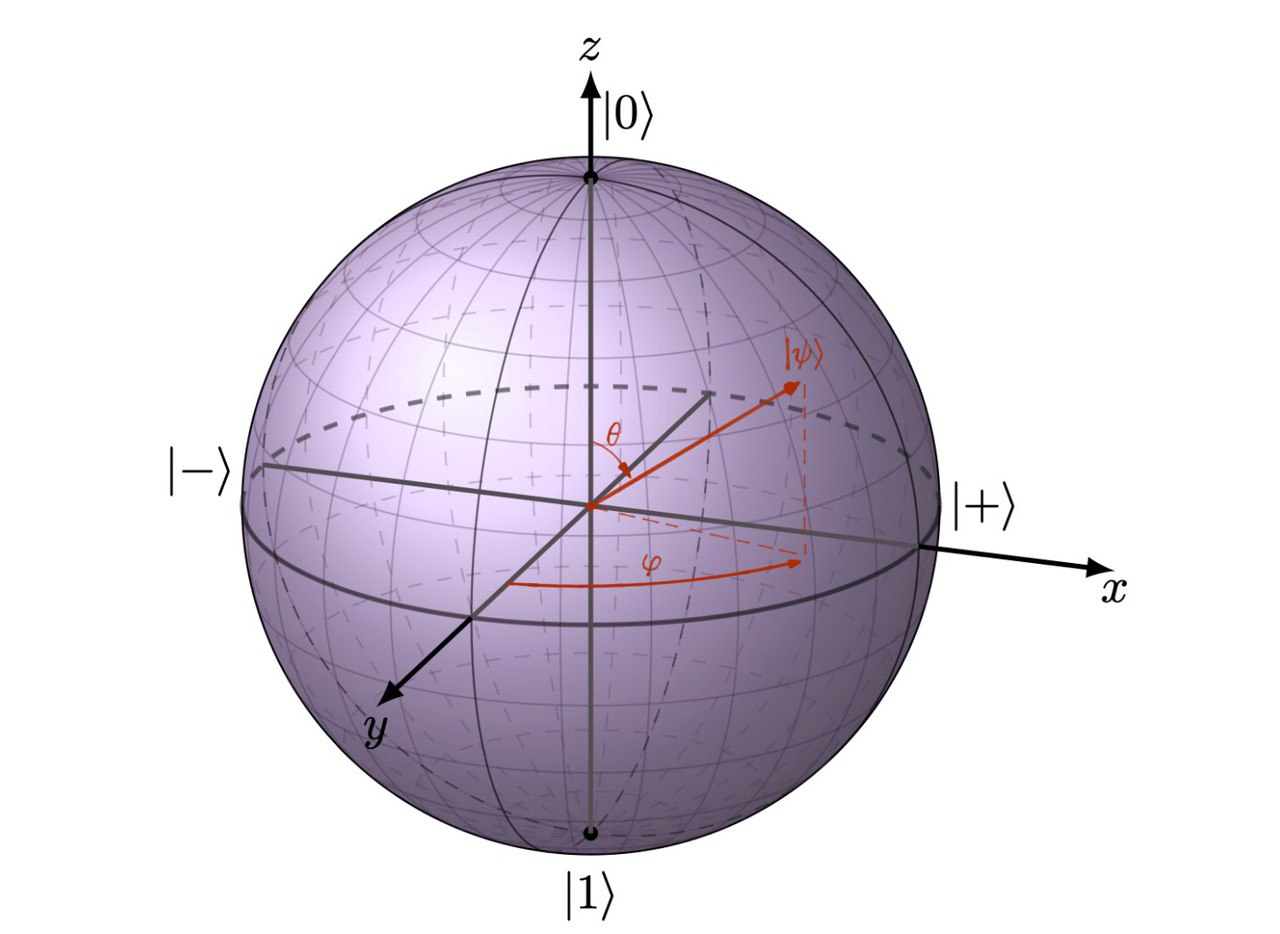
\includegraphics[scale=0.25]{Mainmatter/images/blochhh.jpg}
    \caption{Bloch sphere}
    \label{sphere:bloch}
\end{figure}
This sphere is called the Bloch sphere and provides a useful means of visualizing the state of a single qubit, and often serves as an excellent test for ideas about quantum computation and quantum information.
Many of the operations can be done on a single qubit, through logic gates, and they can be described within the Bloch sphere picture.
However, it must be kept in mind that this intuition is limited because there is no simple generalization of the Bloch sphere known for multiple qubits.

A system of multiple qubits is represented by tensor-product Hilbert spaces; for example, a system composed of two qubits has a state
$|\psi\rangle$ belonging to the tensor product of the Hilbert spaces of the two individual qubits, and we say that $|\psi\rangle \in \mathcal{H}_1 \otimes \mathcal{H}_2$. However, in this and in even larger spaces, there is a fundamental and physically crucial difference between the two kinds of states. There are the so called factorizable states, which can be expressed in the form of tensor product: 
\begin{equation*}
    \ket{\psi} = \left(\alpha_{1}|0\rangle_{1}+\beta_{1}|1\rangle_{1}\right) \otimes[\ldots] \otimes\left(\alpha_{n}|0\rangle_{n}+\beta_{n}|1\rangle_{n}\right)
\end{equation*}
and there are also the  entangled states which are "un-factorizable", i.e the quantum state cannot be factorised as a product of states of its local constituents. 
A perfect example can be provided by considering a two qubits system; a factorizable state is: 
$$
\left|\psi_{f}\right\rangle=(\alpha_1\alpha_2|00\rangle+\alpha_1\beta_2|01\rangle+\beta_1\alpha_2|10\rangle+\beta_1\beta_2|11\rangle)=(\alpha_1|0\rangle+\beta_1|1\rangle) \otimes(\alpha_2|0\rangle+\beta_2|1\rangle)
$$
while an example of entangled state could be:
$$
\left|\psi_{e}\right\rangle=\alpha|00\rangle+\beta|11\rangle.
$$


%A state system of multiple qubits can be expressed as the n-fold tensor product between all the Hilbert space of the single qubit. For example, a system of n qubits lies in $\mathcal{H}=\mathcal{H}_1 \otimes \mathcal{H}_2 \otimes\mathcal{H}_3 \otimes ... \otimes\mathcal{H}_{n-1} \otimes\mathcal{H}_n$.


%The concepts relating to quantum computation and, in particular, the concept of qubits are based on quantum mechanics.
%The physical layer is therefore endowed with properties that cannot be observed in the macroscopic world, such as superposition of states, interference, entanglement and indeterminacy.
Qubit states can be manipulated and transformed in ways that lead to measurement outcomes that depend distinctly on the different properties of the state. 
However, in the end, we cannot measure a qubit in its state of superposition but we can manipulate the amplitudes to get the result which we are looking for.
A quantum computer can create vast multidimensional spaces in which to represent very large problems, solve the problem using the properties of quantum mechanics, some logic gates, and operations. One of the techniques consists in adjusting the amplitude contributions, in fact, if some amplitudes are positive and others are negative, then the contributions can interfere destructively and cancel each other out. %so that the amplitude is zero and the corresponding outcome is never observed;
Likewise, they can interfere constructively and increase the likelihood of a given outcome. The goal in devising an algorithm for a quantum computer is to choreograph a pattern of constructive and destructive interference so that for each wrong answer the contributions to its amplitude cancel each other out, whereas for the right answer the contributions reinforce each other. If you can arrange that, one will see the right answer with a large probability when one measures. The tricky part is to do this without knowing the answer in advance, and faster than you could do it with a classical computer.



Another important question is: how much information can be carried by a qubit?
Paradoxically, a qubit can exist in a continuum of states between the two bases, so there are an infinite number of linear combinations of the orthonormal basis apparently allowing, at least in principle, the representation of all human knowledge in a single qubit.

However, this is an erroneous conclusion by virtue of the behavior of the qubit during measurement. It must be kept in mind, in fact, that the outcome of the measurement of the state of a qubit can only be $\ket{0}$ or $\ket{1}$, with respective probabilities $|\alpha|^2$ and $|\beta|^2$. We can interpret this as the condition that the qubit’s state is normalized to length $1$. 
Moreover, the measurement of the qubit inexorably changes its state, collapsing the superposition state in one of the two specific states represented by the vectors of the computational basis as prescribed by the postulate of measure in quantum mechanics.

Thus, from the measurement of a qubit, it is possible to obtain the same amount of information that can be represented by a classical bit. This result has been proved rigorously by Holevo's Theorem.








There is currently no preferred qubit technology, a variety of physical systems are being explored for use as qubits: the two different polarizations of a photon, as the alignment of a nuclear spin in a uniform magnetic field... 
In contrast, bits in a classical computer are typically realized as the robust on/off states of transistor switches which are differentiated by billions of electrons.
A shortcoming shared by all of these approaches to realize a quantum computer is that it is difficult to sufficiently isolate the qubits from the effects of external noise, meaning errors during quantum computation are inevitable, and quantum error correction codes have been developed in order to protect a qubit from the external noise. After this introduction in \ref{chap:2} I will describe how these codes work. 


\section{Quantum gates}\label{sec:qgate}

Classically one can manipulate a system of bits and make some operations on it, using logic gates in order to solve a certain problem. Analogous to the way a classical computer is built from an electrical circuit containing wires and logic gates, a quantum computer is built from a quantum circuit containing wires and elementary quantum gates to carry around and manipulate the quantum information.
A quantum gate can be represented as an operator acting on the states of one or more qubits, depending on the nature of the gate.
A qubit can be represented as a two-dimensional ket. Thus, the operator algebra acting on those kets is 4-dimensional. 


A quantum gate has to preserve the normalization condition of a state $|\psi\rangle$. Given an operator $\hat{U}$ that transforms $|\psi\rangle \rightarrow\left|\psi^{\prime}\right\rangle$, it follows:
$$
\left\langle\psi^{\prime} \mid \psi^{\prime}\right\rangle =\bra{\psi}\hat{U}^{\dagger} \hat{U}\ket{\psi}=1
$$
Hence, 
$$
 \hat{U}^{\dagger} \hat{U}=\widehat{\mathbb{I}}
$$
Operators satisfying this condition are called unitary operators. This imply that all quantum gates are also reversible, in fact, equation  prove that $\hat{U^{-1}}$ exists and it is equal to $\hat{U}^{\dagger}$, thus:
$$
\hat{U}^{\dagger}\left|\psi^{\prime}\right\rangle=\hat{U}^{\dagger} \hat{U}|\psi\rangle=\hat{\mathbb{I}}|\psi\rangle=|\psi\rangle
$$
If we consider a one qubit system, a suitable basis for these unitary operators acting on the system can be given by the identity matrix and the pauli matrices: 
$$
I=\left(\begin{array}{cc}
1 & 0 \\
0 & 1
\end{array}\right) \quad  \sigma_X=X=\left(\begin{array}{cc}
0 & 1 \\
1 & 0
\end{array}\right) \quad 
\sigma_Y=Y=\left(\begin{array}{cc}
0 & -i \\
i & 0
\end{array}\right) \quad
\sigma_Z=Z=\left(\begin{array}{cc}
1 & 0 \\
0 & -1
\end{array}\right).
$$
All these matrices are unitary and also hermitian, which implies that $\sigma_i=\sigma_i^{-1} \quad \forall i = X,Y,Z$, where $\sigma$ represent one of the 3 pauli matrices. Moreover, the Pauli matrices satisfy the following relations:
$$
\begin{aligned}
\sigma_{i} \sigma_{j} &=\delta_{i j} \mathbb{I}+i \epsilon_{i j k} \sigma_{k} \\
\left[\sigma_{i}, \sigma_{j}\right] &=2 i \epsilon_{i j k} \sigma_{k} \\
\left\{\sigma_{i}, \sigma_{j}\right\} &=2 \delta_{i j} \mathbb{I}
\end{aligned}
$$
where $\epsilon_{i j k}$ is the Levi-Civita symbol, $[\cdot, \cdot]$ is the commutator and $\{\cdot, \cdot\}$ is the
anticommutator.
These 4 matrices provide a basis of the operators acting on a single qubit. It follows that every single qubit operator can be expressed as a linear combination of $I,X,Y,Z$: 
\begin{equation*}
    U = \alpha I+\beta X+\gamma Y+\delta Z \quad \text{with $\alpha,\beta,\gamma,\delta$ complex numbers}.
\end{equation*}
and a multi-qubit operator can be expressed as a tensor product of single qubit operators:
\begin{equation*}
    U = U_1 \otimes U_2 \otimes ... \otimes U_n.
\end{equation*}
Quantum gates are reversible by definition. Thus, the numbers of qubits in input must be the same as the qubits in output, otherwise, the gates are not reversible. An immediate consequence of this property is, for instance, that the classical AND gate, largely used in classical computing, could not have an exact quantum analog.
Among all the quantum gates having as an input a single qubit, the most remarkable for our purpose are the quantum NOT, the Z gate, the Hadamard gate, and the general phase shift gate.
Instead, from all the gates that act on two qubits, the most important one in our context is the controlled-NOT gate.
In what follows we briefly introduce these gates. 

\subsection*{The quantum NOT gate}
In quantum circuits, it is represented by: \begin{figure}[H]
\centering
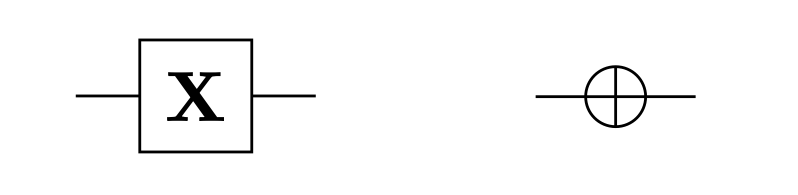
\includegraphics{Mainmatter/images/XGATE.png}
\end{figure}
Using the analogy with the classical NOT gate, which acts on the computational basis changing the state 0 in the state 1 and vice versa, one can suppose that the quantum not has the same action on the computational quantum basis, taking $\ket{0} \to \ket{1}$ and $\ket{1} \to \ket{0}$. It is interesting to see what happen to a state which is a superposition of the quantum basis: 
\begin{equation*}
    NOT \ket{\psi} = NOT(\alpha\ket{0} +\beta\ket{1}) = (\alpha\ket{1} +\beta\ket{0})
\end{equation*}
Thus, we can write down the "truth table", or better the action of the gate on the qubit: 
\begin{table}[h!]
    \centering
    \begin{tabular}{c|c}
         Input & Output \\
          $\ket{0}$ & $\ket{1}$ \\
          $\ket{1}$ & $\ket{0}$
    \end{tabular}
    \caption{Truth table quantum NOT gate}
    \label{tab:not_gate}
\end{table}


It is possible to notice that an operator which acts on a qubit like that is the X Pauli matrix, hence this gate it is also called X-gate.

\subsection*{The Z-gate}
In quantum circuits, this gate it is represented by \begin{figure}[H]
\centering
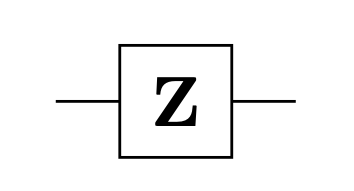
\includegraphics{Mainmatter/images/ZGATE.png}
\end{figure}.
This gate is represented by the Z pauli matrix. The associated "truth table" is: 
\begin{table}[h!]
    \centering
    \begin{tabular}{c|c}
         Input & Output \\
          $\ket{0}$ & $\ket{0}$ \\
          $\ket{1}$ & -$\ket{1}$
    \end{tabular}
    \caption{Caption}
    \label{tab:my_label}
\end{table}


This is a phase shifting in the space spanned by $\ket{0}$ and $\ket{1}$. However it can be understood as a bit-flip gate in other orthonormal basis states. For example, if we consider as computational basis $\ket{+}= \frac{\ket{0} + \ket{1}}{\sqrt{2}}$ and $\ket{-} = \frac{\ket{0} - \ket{1}}{\sqrt{2}}$, with respect to this new base elements, the action of the Z-gate is:
\begin{table}[h!]
    \centering
    \begin{tabular}{c|c}
         Input & Output \\
          $\ket{-}$ & $\ket{+}$ \\
          $\ket{+}$ & $\ket{-}$
    \end{tabular}
    \caption{"Truth table" of Z-gate in the new basis}
    \label{tab:not_gate}
\end{table}



Another interesting observation that can be seen is the action of the X-gate on a generic state $\ket{\psi} = \alpha \ket{+} + \beta \ket{-}$ in this new basis. In this new base the X matrix is: 
\begin{equation*}
    X_{\ket{+},\ket{-}} = M^{-1}X M = \left(\begin{array}{cc}
1 & 0 \\
0 & -1
\end{array}\right)  
\end{equation*}
Hence, the action of X in the new basis is the same as that of operator Z in the old basis.


\subsection*{The general phase-shift gate}
The Z gate is a particular case of the phase rotation gate, which corresponds to a phase shift of $\pi$. In quantum circuits, this gate it is represented by :
\begin{figure}[H]
\centering
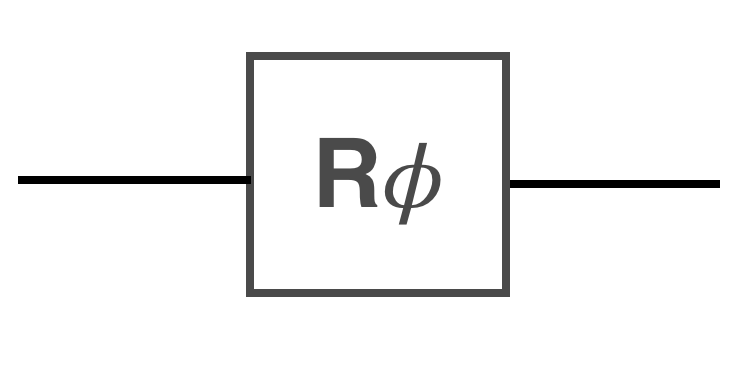
\includegraphics[scale=0.15]{Mainmatter/images/Phase_shift_gate.png}
\end{figure}
The phase-shift gate maps $\ket{0} \to \ket{0}$ and $\ket{1} \to e^{i\phi}\ket{1}$, where $\phi$ is the phase shift. It is possible to notice that if $\phi=\pi$. Thus, $e^{i\pi}=-1$ obtaining the Z-pauli matrix. The phase-shift $\phi$ can assume all the value from 0 to $2\pi$.

The probability of measuring a $\ket{0}$ or $\ket{1}$ is unchanged after applying this gate, however it modifies the phase of the quantum state.

The associated truth table is: 
\begin{table}[h!]
    \centering
    \begin{tabular}{c|c}
         Input & Output \\
          $\ket{0}$ & $\ket{0}$ \\
          $\ket{1}$ & $e^{i\phi}\ket{1}$
    \end{tabular}
    \caption{Truth table of R-gate}
    \label{tab:rotationgate}
\end{table}

The phase shift gate is represented by the matrix:
\begin{equation*}
     R_{\phi}=  \left(\begin{array}{cc}
1 & 0 \\
0 & e^{i\phi}
\end{array}\right)  .
\end{equation*}
But, sometimes in literature a different convention is adopted. In the following thesis I will specify always which one I use. 
To get an example of the other convention 
is usually represented with the $\theta$ angle.
\begin{equation*}
     R_{\theta / 2}=  \left(\begin{array}{cc}
1 & 0 \\
0 & e^{i\theta}
\end{array}\right)  .
\end{equation*}



\subsection*{The Hadamard gate}
In quantum circuits, this gate is represented by:
\begin{figure}[H]
\centering
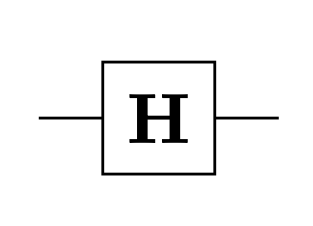
\includegraphics{Mainmatter/images/Hadamard_GAte.png}
\end{figure}
The hadamard gate acts on a single qubit creating a superposition if a basis state is given. It maps $\ket{0} \to \frac{\ket{0} + \ket{1}}{\sqrt{2}} = \ket{+}$  and  $\ket{1} \to \frac{\ket{0} - \ket{1}}{\sqrt{2}} = \ket{-}$. 
In particular, it corresponds exactly to the change of basis matrix from the $\{|0\rangle,|1\rangle\}$ to the $\{|+\rangle,|-\rangle\}$ bases and, thanks to the fact that it is self-reversible, also vice-versa. Its truth table is: 
\begin{table}[h!]
    \centering
    \begin{tabular}{cc}
\hline Input & Output \\
\hline$|0\rangle$ & $|+\rangle$ \\
$|1\rangle$ & $|-\rangle$ \\
\hline
\end{tabular}
    \caption{Caption}
    \label{tab:my_label}
\end{table}

And its matrix representation in the computational basis $\ket{0},\ket{1}$ is: 
\begin{equation*}
    H = \frac{1}{\sqrt{2}} \left(\begin{array}{cc}
1 & 1 \\
1 & -1
\end{array}\right)  
\end{equation*}

\subsection*{The controlled-NOT gate}
The CNOT gate acts on 2 qubits inverting the second qubit $\oplus$ (the target qubit) if and only if the first qubit $\Bigcdot$ (the control qubit ) is $\ket{1}$. In quantum circuit, it is represented by: 
\begin{figure}[H]
\centering
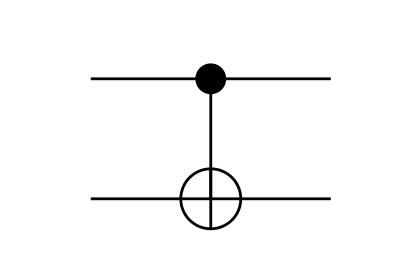
\includegraphics{Mainmatter/images/CNOT_gate.png}
\end{figure}
By being binary its truth table traces 4 different possible input scenarios: 
\begin{table}[h!]
    \centering
    \begin{tabular}{cc|cc}
    \hline
    \multicolumn{4}{c}{Input \quad \quad \quad \quad  \quad     Output } \\
    \hline Control& Target & Control & Target\\
\hline$|0\rangle$ & $\ket{0}$ & $\ket{0}$&$\ket{0}$\\
$|0\rangle$ & $|1\rangle$ &$|0\rangle$ & $|1\rangle$ \\
$|1\rangle$ & $\ket{0}$ & $\ket{1}$&$\ket{1}$ \\
$|1\rangle$ & $\ket{1}$ & $\ket{1}$&$\ket{0}$\\
\hline
\end{tabular}
    \caption{Action of the CNOT gate}
    \label{tab:my_label}
\end{table}
and so does the matrix representation which, this time, is based on a 4 × 4 matrix: 

\begin{equation*}
    CNOT =  \left(\begin{array}{cccc}
1 & 0 & 0 & 0\\
0 & 1 & 0 & 0\\
0 & 0 & 0 & 1\\
0 & 0 & 1 & 0\\
\end{array}\right)  
\end{equation*}
This gate is widely used to creates
entangled states. As an example, consider this circuit: 
\begin{figure}[h!]
    \centering
    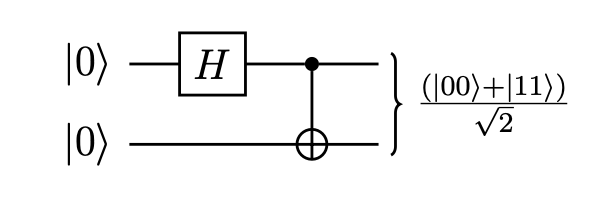
\includegraphics[scale=0.5]{Mainmatter/images/CNOT_entangled.png}
\end{figure}


where the final state is also known as $\ket{\Phi^+}$ Bell state.
Starting from the second chapter, we are going to use these gates to build quantum circuits for quantum error correction codes. Instead, in the last chapter I will focus more on how to make these gates more reliable. 






\section{Density operator}
The formalism for pure quantum states does not immediately allow for a formalisation of ignorance or missing knowledge about the state of a quantum system.
Suppose that the mechanism that generates replicas of the same system does not always produce the same pure state but produces several of them. We do not exactly know in what state our system is, but instead we are given with some possible states $\ket{\psi_{\lambda}}$ with probability $p_{\lambda}$. The set (or ensemble) of replicas corresponds to a mixture of pure states. This mixture is called mixed state or mixed ensemble. 
%I want to emphasise that the mixture cannot be described as a superposition of the orthonormal basis in the Hilbert space that characterise the system.
In quantum mechanics, the density matrix operator is an useful tool to describe an ensemble of quantum states. It is a generalization of the more usual state vectors approach, which can only describe pure states. 
A pure state is by definition:
\begin{equation}
    \ket{\psi} = \sum_j c_j \ket{\psi_j}
\end{equation}
where the coefficients $c_j$ are complex numbers $\ket{\psi_j}$ are the eigenvectors of an observable\footnote{for instance, in quantum computing the most common observable is the spin along the z axes $S_z$, which indicates the computational basis $\ket{0}$ and $\ket{1}$} that constitute a complete orthonormal basis in the Hilbert space for the states describing the system.
% In fact, a pure quantum state can be represented by a ray in a Hilbert space over the complex numbers, while mixed states are represented by density matrices, which are positive semidefinite operators that act on Hilbert spaces.


% Using density operator we can represent mixed states (ensemble of pure states), which no longer can be expressed as kets but are characterized by the density operator. 
%Mixed states arise in quantum mechanics in different situations. For example, fluactuation in experiment...
%or if the same state goes through a noisy channel, at the end of the channel we could have different states with different probability p, ... 


Instead, we call $\{p_{\lambda}, \ket{\psi_{\lambda}} \}$ an ensemble of pure state, where $p_{\lambda}$ are real numbers that indicate the classical probability to pick up a pure state $\ket{\psi_{\lambda}}$ from the ensemble. Recall the fact that the probabilities $p_{\lambda}$ are real numbers without a phase between them. While the coefficients of a decomposition are related by a phase. 
%We can represent a mixed state in the bloch sphere, for instance $\{(p_0=\frac{1}{2})|\ket{0}, (p_1=\frac{1}{2})|\ket{1}\}$ can be seen as a new bloch sphere with halved radius. 

Describing the state of a quantum system with such probabilistic mixtures opens up the possibility of having non-reversible evolution. 

For instance, in the case of a qubit, we might start in a certain state $\ket{\psi} = a\ket{\psi}+ b\ket{\psi}$ with unit probability, but if we measure the state the knowledge is lost or transferred to another register or ignored such that the final probabilistic mixture describing the qubit’s state is $\{(p_0=\frac{1}{2})|\ket{0}, (p_1=\frac{1}{2})|\ket{1}\}$. That is, we have a uniform probability distribution over the computational basis states. Certainly, this evolution is not reversible as the final probabilistic mixture alone does not allow for a reconstruction of the initial state, because the same measurements results can be given by a mixture of states ($\{(p_0=\frac{1}{2})|\ket{0}, (p_1=\frac{1}{2})|\ket{1}\}$) or by a single state in a superposition ($\ket{\psi} = a\ket{\psi}+ b\ket{\psi}$).


In the light of the above, the density operator or density matrix of the system is defined: 
\begin{equation}
    \rho = \sum_{\lambda} p_{\lambda} \ket{\psi_{\lambda}}\bra{\psi_{\lambda}} 
    \label{eq:density}
\end{equation}
with the constrain that $\sum_{\lambda} p_{\lambda}=1$
. If the system is composed of only one pure state, the density matrix is: 
\begin{equation}
    \rho = \ket{\psi}\bra{\psi}
\end{equation}
%The matrix representation depends on the basis that we chose, for example, a density matrix that represent a single qubit can be represented with $\ket{0},\ket{1}$ as a basis: 
% \begin{equation}
%      \rho_{mn} = \bra{m}\ket{\psi}\bra{\psi}\ket{n}= \begin{pmatrix} a \\ b \end{pmatrix} 
%   \begin{pmatrix} a \\ b \end{pmatrix}^{\dagger} = \begin{pmatrix} |a|^2 & ab^* \\ ba^* & |b|^2  \end{pmatrix}
% \end{equation}
A way to estimate how pure a system is, one can compute the trace of $\rho^2$ since this is always less than 1. In fact: 
\begin{equation*}
    Tr(\rho^2) = Tr(\rho^2_{diag}) = \sum_{\lambda}p^2_{\lambda} \leq 1
\end{equation*}
If the probabilities $p_{\lambda}$ are all zero except the one for some $\lambda'$ for which $p_{\lambda'}=1$, then the ensemble corresponds to a set of replicas of a system in the same pure state $\ket{\psi_{\lambda}}$.
To evaluate the expectation value of a generic observable $Q$ over this ensemble, we have to add up the expectation values we obtain for each pure state, weighing them with the probabilities $p_{\lambda}$:
$$
\langle Q\rangle_{mix}=\sum_{\lambda} p_{\lambda}\left\langle\psi_{\lambda}|Q| \psi_{\lambda}\right\rangle=\sum_{\lambda} p_{\lambda} \sum_{i, j} c_{i}^{*(\lambda)} c_{j}^{(\lambda)}\left\langle a_{i}|Q| a_{j}\right\rangle
$$
where the coefficients  $c_{j}^{(p)}=\left\langle a_{j} \mid \psi_{\lambda}\right\rangle$ are those of the state decomposition $\left|\psi_{\lambda}\right\rangle$ on the basis of the eigenvectors of $A$ (observable that characterises the system, for a qubit can be the spin along the z direction, which gives $\ket{0}$ and $\ket{1}$ as basis vector).
$$
\begin{aligned}
\langle Q\rangle_{mix} &=\sum_{\lambda} p_{\lambda} \sum_{i, j} \left\langle a_{i}|Q| a_{j}\right\rangle  \left\langle\psi_{\lambda} \mid a_{i}\right\rangle\left\langle a_{j} \mid \psi_{\lambda}\right\rangle\\
&=\sum_{i, j} \left\langle a_{i}|Q| a_{j}\right\rangle \left(\sum_{\lambda} p_{\lambda} \left\langle a_{j} \mid \psi_{\lambda}\right\rangle\left\langle\psi_{\lambda} \mid a_{i}\right\rangle\right) \\
&=tr(Q \rho)
\end{aligned}
$$

% Moreover, for each measurement that can be defined, the probability distribution over the outcomes of that measurement can be computed from the density operator using the Born rule\footnote{The Born rule states that if an observable corresponding to a self-adjoint operator $A$ with discrete spectrum is measured in a system with normalized wave function $|\psi\rangle$, then:


%  1) the measured result will be one of the eigenvalues $a$ of $A$
 
 
%     2) the probability of measuring a given eigenvalue $a_{i}$ will equal $\left\langle\psi\left|P_{i}\right| \psi\right\rangle$, where $P_{i}$ is the projection onto the eigenspace of $A$ corresponding to $a_{i}$
% saying that probability is equal to the amplitude-squared. Equivalently, the probability can be written as $|\braket{ a_{i} \mid \psi}|^{2}$).}

% When performing a measurement $\left\{\Pi_{x}\right\}_{x}$ on a probabilistic mixture we expect to obtain an outcome $x$ with a certain probability
%   $$
%   .\operatorname{Pr}\left[x \mid\left\{\left(p_{\lambda},\ket{\psi_{\lambda}}\right)\right\}_{\lambda}\right]=\sum_{\lambda} \operatorname{Pr}\left[\ket{\psi_{\lambda}}\right] \cdot \operatorname{Pr}\left[x|| \psi_{\lambda}\right\rangle]
%  $$
%  This is the formula for conditional probabilities, where $\operatorname{Pr}\left[\ket{\psi_{\lambda}}\right]=p_{\lambda}$ is the probability to find the system in $\ket{\psi_{\lambda}}$ and $\left.\operatorname{Pr}\left[x|| \psi_{\lambda}\right\rangle\right]=\left\langle\psi_{\lambda}\left|\Pi_{x}\right| \psi_{\lambda}\right\rangle$ is the probability to obtain outcome $x$ given that the quantum system's state is $\ket{\psi_{\lambda}} .$ Hence the probability of obtaining outcome $x$ can be rewritten as
%  $$
%  \operatorname{Pr}\left[x \mid\left\{\left(p_{\lambda},\ket{\psi_{\lambda}}\right)\right\}_{\lambda}\right]=\sum_{\lambda} p_{\lambda}\left\langle\psi_{\lambda}\left|\Pi_{x}\right| \psi_{\lambda}\right\rangle= \operatorname{tr}\left(\Pi_{x}\rho\right)
%  $$
%  where $\rho$  is the density operator, and 
%  $\Pi_x$ is the projection operator onto the basis vector corresponding to the measurement outcome $x$.
%  A measurement upon a quantum system will generally bring about a change of the quantum state of that system. We can ....
 %where we used the definition of the trace, in the second equality.
 
 %Since the trace is a linear operator, we can bring this formula into its final form
%  $$
%  \operatorname{Pr}\left[x \mid\left\{\left(p_{\lambda},\ket{\psi_{\lambda}}\right)\right\}_{\lambda}\right]=\operatorname{tr}\left(\Pi_{x} \sum_{\lambda} p_{\lambda}\left|\psi_{\lambda} X \psi_{\lambda}\right|\right)
%  $$
% We conclude that what determines the outcome probabilities of a given measurement is the density operator \ref{eq:density}.
Another advantage of working with the density matrix notation is that, when dealing with composite systems, for example system and environment, it provides a practical way to extract the state of each subsystem, even if they are entangled. This is done in the form of what is known as the reduced density matrix.
Consider a quantum system composed of subsystems $A$ and $B$, and fully described by the density matrix $\rho_{A B}$. The reduced density matrix of subsystem $A$ is then given by:
$$
\rho_{A}=\operatorname{Tr}_{B}\left(\rho_{A B}\right)
$$
Here, $\operatorname{Tr}_{B}$ is an operation known as the partial trace, which is defined as:
$$
\operatorname{Tr}_{B}\left(\left|\psi_{u}\right\rangle\left\langle\psi_{v}|\otimes| \varphi_{u}\right\rangle\left\langle\varphi_{v}\right|\right) \equiv\left|\psi_{u}\right\rangle\left\langle\psi_{v}\right| \operatorname{Tr}\left(\left|\varphi_{u}\right\rangle\left\langle\varphi_{v}\right|\right)
$$
$\left|\psi_{u}\right\rangle$ and $\left|\psi_{v}\right\rangle$ are arbitrary states in the subspace of $A$, and $\left|\varphi_{u}\right\rangle$ and $\left|\varphi_{v}\right\rangle$ arbitrary states in the subspace of $B$. Tr is the standard trace operation, which for two arbitrary states $\operatorname{Tr}\left(\left|\varphi_{u}\right\rangle\left\langle\varphi_{v}\right|\right)=\left\langle\varphi_{v} \mid \varphi_{u}\right\rangle$. 
As an example, let us reconsider the pure entangled state:
$$
\left|\Phi^{+}_{A B}\right\rangle=\frac{1}{\sqrt{2}}\left(\left|0_{A} 0_{B}\right\rangle+\left|1_{A} 1_{B}\right\rangle\right)
$$
This system is then composed of single-qubit subsystem $A$ with basis vectors $\left\{\left|\psi_{1}\right\rangle,\left|\psi_{2}\right\rangle\right\}=\left\{\left|0_{A}\right\rangle,\left|1_{A}\right\rangle\right\}$, and single-qubit subsystem $B$ with basis vectors $\left\{\left|\varphi_{1}\right\rangle,\left|\varphi_{2}\right\rangle\right\}=\left\{\left|0_{B}\right\rangle,\left|1_{B}\right\rangle\right\} .$ We know that this system is not separable; however, by using the reduced density matrix, we can find a full description for subsystems $A$ and $B$ as follows.

The density matrix of our state $\left|\Phi^{+}_{A B}\right\rangle$ can be expressed in terms of outer products of the basis vectors:
$$
\rho_{A B}=\left|\psi_{A B}\right\rangle\left\langle\psi_{A B}\right|=\frac{1}{2}\left[\left|0_{A} 0_{B}\right\rangle\left\langle 0_{A} 0_{B}|+| 0_{A} 0_{B}\right\rangle\left\langle 1_{A} 1_{B}|+| 1_{A} 1_{B}\right\rangle\left\langle 0_{A} 0_{B}|+| 1_{A} 1_{B}\right\rangle\left\langle 1_{A} 1_{B}\right|\right]
$$.
Then, for example, the reduced density matrix for the subsystem $B$ is:
\begin{align*}
\rho_{B} &=\operatorname{Tr}_{A}\left(\rho_{A B}\right) \\
&=\frac{1}{2}\left[\operatorname{Tr}_{A}\left(\left|0_{A} 0_{B}\right\rangle\left\langle 0_{A} 0_{B}\right|\right)+\operatorname{Tr}_{A}\left(\left|0_{A} 0_{B}\right\rangle\left\langle 1_{A} 1_{B}\right|\right)+\operatorname{Tr}_{A}\left(\left|1_{A} 1_{B}\right\rangle\left\langle 0_{A} 0_{B}\right|\right)+\operatorname{Tr}_{A}\left(\left|1_{A} 1_{B}\right\rangle\left\langle 1_{A} 1_{B}\right|\right)\right] \\
&=\frac{1}{2}[\operatorname{Tr}\left(\ket{0_A}\bra{0_A}\right)\ket{0_B}\bra{0_B}] +
\operatorname{Tr}\left(\ket{0_A}\bra{1_A}\right)\ket{0_B}\bra{1_B} + 
\operatorname{Tr}\left(\ket{1_A}\bra{0_A}\right)\ket{1_B}\bra{0_B}+ \\
&+ \operatorname{Tr}\left(\ket{1_A}\bra{1_A}\right)\ket{1_B}\bra{1_B}
\\
 &=\frac{1}{2}\left[\left\langle 0_{A} \mid 0_{A}\right\rangle\left|0_{B}\right\rangle\left\langle 0_{B}\left|+\left\langle 1_{A} \mid 0_{A}\right\rangle\right| 0_{B}\right\rangle\left\langle 1_{B}\left|+\left\langle 0_{A} \mid 1_{A}\right\rangle\right| 1_{B}\right\rangle\left\langle 0_{B}\left|+\left\langle 1_{A} \mid 1_{A}\right\rangle\right| 1_{B}\right\rangle\left\langle 1_{B}\right|\right] \\
 &=\frac{1}{2}\left[\left|0_{B}\right\rangle\left\langle 0_{B}|+| 1_{B}\right\rangle\left\langle 1_{B}\right|\right] =\frac{I}{2}
\end{align*}

It is worth mentioning that so far we have described the concept of partial trace for a bipartite (two-party) system, but this can be generalized for multi-party systems.




Moreover, Using the density operator formalism we can successfully study the evolution of a closed quantum system, we will describe it better considering different type of noise and evolution in the next sections. The time evolution is usually described by the unitary operator $U(t,t_0)$. If the system was initially in the state $\ket{\psi_{\lambda}}$ with probability $\psi_{\lambda}$ then after the evolution has occurred the system will be in the state $U\ket{\psi_{\lambda}}$ with the same classical probability . Thus, the evolution of the density operator is described by the equation: 
\begin{equation}
    \rho = \sum_{\lambda} p_{\lambda} U\ket{\psi_{\lambda}}\bra{\psi_{\lambda}}U^{\dagger} = U\rho U^{\dagger}
\end{equation}
%Moreover, using the density operator language we can describe the  measurements on the 
%It is important the difference between the weight or the classical probability from the coefficients of a superposition. 
The density operator approach really excels for two applications: the description of quantum systems whose state is not known, and the description of subsystems of a composite. To write this section I was helped by : \cite{Dalfovo}\cite{Chuang}\cite{Hauke}\cite{Qiskit}


\section{Quantum errors: Noise and Decoherence}
The Schrödinger equation
$$
i \hbar \frac{d|\psi\rangle}{d t}=H|\psi\rangle
$$
describes the evolution of quantum systems in isolation, where $|\psi\rangle$ is the state vector. These closed systems have a well-defined Hamiltonian operator $H$, which gives complete information about how these systems evolve. The resulting evolution is unitary: the evolution of the state is given by a linear map $|\psi(0)\rangle \rightarrow|\psi(t)\rangle=U|\psi(0)\rangle$ where $U^{\dagger} U=$ $U U^{\dagger}=I$. Note that these Hamiltonians may "come from outside" the system; for instance, we can turn external fields on and off, shine lasers, etc. What makes a quantum system closed is that it doesn't act back on the external world. The external fields, lasers, etc., can all be treated as classical potentials.

The unfortunate reality is that this idealization is a fiction. All real quantum systems interact with the outside world, at least weakly; and the existence of interactions, which allow us to manipulate a system, also allow the system to interact with the external environment. This environmental interaction is called decoherence.

One can model the dynamics of a register of qubits with its surroundings. We imagine the system immersed into its environment (often called bath) and the whole (quantum register plus environment) as a closed system described in a general way by the following Hamiltonian:
$$
H=H_{S} \otimes I_{B}+I_{S} \otimes H_{B}+H_{\mathcal{I}}
$$
where $H_{S}\left(H_{B}\right)$ (the system (bath) Hamiltonian) acts on the system (bath) Hilbert space $\mathcal{H}_{S}$ $\left(\mathcal{H}_{B}\right), I_{S}\left(I_{B}\right)$ is the identity operator on the system (bath) Hilbert space, and $H_{I}$, which acts on both the system and bath Hilbert spaces $\mathcal{H}_{S} \otimes \mathcal{H}_{B}$, is the interaction Hamiltonian containing all the nontrivial couplings between system and bath. In general $H_{\mathcal{I}}$ can be written as a sum of operators which act separately on the system $\left(S_{\alpha}\right.$) and on the bath $\left(B_{\alpha}\right.$):
$$
H_{I}=\sum_{\alpha} S_{\alpha} \otimes B_{\alpha}
$$
(Note that this decomposition is not necessarily unique). In the absence of an interaction Hamiltonian $\left(H_{\mathcal{I}}=0\right)$, the evolution of the system and the bath are separately unitary: $\mathbf{U}(t)=\exp (-i \frac{H}{\hbar} t)=\exp \left(-i \frac{H_{S}}{\hbar} t\right) \otimes \exp \left(-i \frac{H_{B}}{\hbar} t\right)$ . Information that has been encoded (mapped) into states of the system Hilbert space remains encoded in the system Hilbert space if $H_{\mathcal{I}}=0$.
 However in the case when the interaction Hamiltonian contains nontrivial couplings between the system and the environment ($H_{\mathcal{I}}\neq 0$),decoherence happens. %information that has been encoded over the system Hilbert space does not remain encoded over solely the system Hilbert space but spreads out instead into the combined system and bath Hilbert space as the time evolution proceeds.

Two things happen in decoherence. First, random influences from the outside can perturb the system's evolution, as if some random Hamiltonian was turned on, in addition to the usual Hamiltonian. Second, the interaction between the system and environment can cause information about the system to leak into the environment. This information leakage leaves the system correlated with the environment. In fact, the information that was carried by the system before, then a certain quantity is spread out also in the environment, the No-hiding theorem show how this property works. The effect on the system is as if unwanted measurements have been performed (without, in general, our knowing the measurement results).
In fact, these two processes generally both occur, and the practical effects of them often look similar. Indeed, in quantum mechanics there is no sharp distinction between them. If decoherence persists long enough, it is possible for all information about the original state of the system to be lost. In the shorter term, decoherence can destroy quantum effects such as interference and entanglement (on which quantum information processing depends).

In general, we can study the evolution of an isolate quantum systems subjected to decoherence and other sources of noise using quantum states, but as already said in the previous section, the state vector approach does not immediately allow for a formalisation of ignorance or missing knowledge, hence a more general description can be done using the density matrix formalism. This allows for the possibility to study mixed states (i.e., contains uncertainties that represent missing information) rather than only pure (isolated and perfectly known).
Then, once the initial state is represented by density operator we can find a function with certain properties that describes the evolution of the density operator.
Maps that represent this evolution must preserve these properties: they are completely positive, trace-preserving and map density matrix into density matrix.
A suitable ensemble of maps that satisfy this properties are called CPTP maps. These maps can be written as
$$
\rho' = \mathcal{E}(\rho) \rightarrow \sum_{\mu} K_{\mu} \rho K_{\mu}^{\dagger} \quad \text { with } \sum_{\mu} K_{\mu}^{\dagger} K_{\mu}=I
$$
where the $K_{\mu}$ are $N \times N$ matrices ($N$ being the dimension of the Hilbert space) and are called Kraus operators. 
In general, the Kraus decomposition of a CPTP map is not unique, but one can approximately think of the map as the state $|\psi\rangle$ being multiplied by one of the operators $K_{\mu}$ chosen at random with probability $p_{\mu}=\bra{\psi} K_{\mu}^{\dagger} K_{\mu}\ket{\psi} .$ Since one does not know which operator has multiplied the state, one uses a mixture of all of them.

In a similar way, if an unknown influence is applied to the quantum system from the outside, we can model that as a set of unitaries $\left\{A_{\mu}\right\}$ that occur with respective probabilities $\left\{p_{\mu}\right\}$. Here, again, one would describe the state of the system as a mixture of all possible evolved states:
$$
\rho \rightarrow \rho^{\prime}=\sum_{\mu} p_{\mu} A_{\mu} \rho A_{\mu}^{\dagger}, \quad \sum_{\mu} p_{\mu}=1
$$
In this case again we have a CPTP map, and we can define the Kraus operators to be $K_{\mu} \equiv \sqrt{p_{\mu}} A_{\mu} .$ Note that the randomness in the unitary evolution need not be due to outside influence:
it could also be from uncertainty of the Hamiltonian, due to imperfect control of the system or any other reason. CPTP maps give a unified description of all possible sources of Markovian noise\footnote{ Markovian dynamics means is a limit or approximation in which the recent details don't matter, that is, the environment is "memoryless" and does not contain information about the history of the system. This is good because it allows to write an equation for $\rho(t)$ that depends only on $\rho(t)$, and not on, say, $\rho\left(t-t^{\prime}\right)$. This is called "Time local" equation and is much easier to handle.}, and in quantum information science one does not usually make a sharp distinction between different noise sources. 




\section{Fidelity}
In comunication problems we would know how much information is preserved by some process. We would like to compare the initial message and the final message after the effect of noise. 
A quantity that can represent how much two states are similar is the fidelity. 
Hence, it is possible to use the fidelity as an appropriate measure of the quality of a recovered code.
A clever way to define the fidelity is to use the desity matrix formalism.
Fidelity is the overlap between the final state $\rho_f$ of a system $\rho$ and the original state $\ket{\psi}$.
If the combined operator consisting of an interaction with the environment followed by a recovery operation is given by $\mathcal{A}=\left\{A_{0}=\mathcal{R}_0E_0, \ldots\right\}$, then the fidelity is
$$
\mathcal{F}\left(\rho_f,\ket{\psi}_i\right)=\bra{\psi_i}\rho_{f}\ket{\psi_i}=\sum_{a}\bra{\psi_i}A_{a}\ket{\psi_i}\bra{\psi_i}A_{a}^{\dagger}\ket{\psi_i} .
$$
It gives the probability that the final state would pass a test checking whether it agrees with the initial state. As we are thinking of encoding arbitrary states, we do not know in advance the state that will be used. We therefore use the minimum fidelity (that is the worst case fidelity)
\begin{equation}
\mathcal{F}_{\min }=\min _{|\psi\rangle}\left\langle\psi\left|\rho_{f}\right| \psi\right\rangle .
\end{equation}
The best quantum code maximizes $\mathcal{F}_{\min }$. 


A quantum communication channel can be use to transmit the state $\ket{\psi}$ from one location to another. No channel is ever perfect, so the action of the channel is described by a quantum operation $\mathcal{E}$ on $\rho=\ket{\psi}\bra{\psi}$. A way to quantify how likely I get $\ket{\psi}$ at the end of the channel is the fidelity. 
Let's take an example of a noisy channel: the depolarising channel. This channel leaves the qubit untouched with probability $1-p$ and with probability $\frac{p}{3}$ one of these 3 error $\{X,Y,Z\}$ can act on the qubit: 
\begin{equation}
    \rho'=\mathcal{D}(\rho) = (1-p)\rho + \frac{p}{3}\left(X\rho X +Y \rho Y+Z \rho Z\right)
\end{equation}
We can write the expression differently: 
$$
\begin{aligned}
\rho^{\prime} &=\frac{p}{3}(X \rho X+Y \rho Y+Z \rho Z)+(1-p) \rho \\
&=\frac{p}{3}(\rho+X \rho X+Y \rho Y+Z \rho Z)+\left(1-\frac{4 p}{3}\right) \rho \\
\end{aligned}
$$
We can simplify the expression more, we can use the following relation\footnote{It is straightforward to calculate that $\mathcal{E}(I)=I$ and $\mathcal{E}(X)=\mathcal{E}(Y)=\mathcal{E}(Z)=0$. However, $I, X, Y, Z$ form a basis of $2\times2$ matrices, so any $\rho$ can be written as $\rho=a I+b X+c Y+d Z$ and then $\mathcal{E}(\rho)=a I$. If $\rho$ is a density matrix then $a=\frac{1}{2}$ and $\mathcal{E}(\rho)=I / 2$. This means that $\mathcal{E}$ maps a pure state into a mixed state, for example $\mathcal{E}(\ket{0}\bra{0}) =\frac{1}{2}(\ket{0}\bra{0} + \ket{1}\bra{1})$}: 
$$
\mathcal{E}(\rho)=\frac{1}{4}(\rho+X \rho X+Y \rho Y+Z \rho Z)=\frac{I}{2}
$$
We can use this result to extract the term proportional to the identity: 
$$
\begin{aligned}
&=\frac{4 p}{3} \frac{I}{2}+\left(1-\frac{4 p}{3}\right) \rho \\
&=\lambda \frac{I}{2}+(1-\lambda) \rho
\end{aligned}
$$
The $p \in[0,1]$ is the Pauli error probability and $\lambda=\frac{4 p}{3} \in\left[0, \frac{4}{3}\right]$ is the depolarization parameter.These two parameters are different because the maximally mixed state $I / 2$ and $(X \rho X+Y \rho Y+Z \rho Z) / 3$ are different states.
From this we can calculate the fidelity between the initial and final mixed state: 
\begin{align*}
    \mathcal{F}(\ket{\psi},\rho') = \text{min}_{\ket{\psi}} &= \bra{\psi}\rho'\ket{\psi} \\
    &= \bra{\psi}(\lambda \frac{I}{2}+(1-\lambda) \ket{\psi}\bra{\psi})\ket{\psi} \\
    &= \frac{\lambda}{2} + (1-\lambda) = 1-\frac{2}{3}p 
\end{align*}
This result agrees well with our intuition the higher the probability $p$ of depolarizing, the lower the fidelity of the final state with the initial state. Provided $p$ is very small the fidelity is close to one, and the state $\mathcal{E}(\rho)$ is practically indistinguishable from the initial state. More examples can be done using different channels in the same way.


So far, we looked only when the state sent into the channel is not entangled, but in quantum error correcting code in order to protect a qubit we have to entangle it. 
The states to be protected involve a subset of entangled qubits. This means that in discussions of fidelity and error, the whole state, not just the component being protected, must be considered.
The worst case fidelity for such states is referred to as the entangled state fidelity to distinguish it from the pure state fidelity introduced earlier.
If the pure state fidelity after recovery of the coded subsystem is one, then the entangled state fidelity is one also; it does not matter if the state is pure or if it is entangled with other systems. This observation is invalid if we have imperfect fidelity.
%We can also characterize the channel by introducing a reference qubit $R$ and describing how a maximally-entangled state of the two qubits $RA$ evolves, when the channel acts only on $A$. There are four mutually orthogonal maximally entangled states, They also form a basis and are called Bell's states. 
%If the initial state is $\left|\phi^{+}\right\rangle_{R A}$, then when the depolarizing channel acts on qubit $A$, the entangled state evolves as
% $$
% \left|\phi^{+}\right\rangle\left\langle\phi^{+}|\mapsto(1-p)| \phi^{+}\right\rangle\left\langle\phi^{+}\right|+\frac{p}{3}\left(\left|\psi^{+}\right\rangle\left\langle\psi^{+}|+| \psi^{-}\right\rangle\left\langle\psi^{-}|+| \phi^{-}\right\rangle\left\langle\phi^{-}\right|\right) .
% $$
Consider a quantum system of combined two quantum subsystems labeled
as $A$ and $B$. The state of $A$ is assumed to be entangled in some way with the external world that we indicates with $B$. Suppose the joint system $AB$ initially is prepared in a general state $\rho_{i}=\ket{\psi_{AB}}\bra{\psi_{AB}}$. This is an entangled state, and we would like to know how well an entangled state is preserved after the action of noise.
Assume that only the subsystem $A$ is affected by the noisy channel with
some evolution described by a quantum operation $\mathcal{E} = \{E_a\}$, for example it can be a bit flip with probability $p_a$. While the subsystem $B$
is dynamically isolated. In this case, the overall dynamics of the joint system $AB$ is described by the quantum operation $\mathcal{E} \otimes I$, where $I$ here is the identity operator acting on the subsystem $B$. Thus the final state of the joint system is given by the density operator $\rho_{\mathrm{f}}= \mathcal{E}\left(\rho_{\mathrm{i}}\right) \otimes I $.
Such as for the isolated state, we can compute the fidelity for an entangled state $\mathcal{F}_e$ as well.
\begin{equation}
\mathcal{F}_{e}(\ket{\psi_{AB}},\rho_f)=\min _{\left|\psi_{AB}\right\rangle }\left\langle\psi_{AB}\left|\rho_f\right| \psi_{AB}\right\rangle
\label{eq:entfidel}
\end{equation}
The $\mathcal{F}_e$, in fact, takes its value in the interval $[0, 1]$, where values close to 1 are supposed to imply that the entanglement is well preserved and values close to $0$ indicate that the entanglement is mostly destroyed.
Using the operation sum representation the action of noise on the initial state is :
\begin{equation*}
\rho_f=(\mathcal{E}\otimes I)(\rho)=\sum_{a} E_a\ket{\psi_{AB}}\bra{\psi_{AB}} E_a^{\dagger}\end{equation*}
Then, we can substitute this in eq(\ref{eq:entfidel}): 
\begin{align*}
    \mathcal{F}_e&=\text{min}_{\psi_{AB}} \sum_a  \bra{\psi_{AB}}E_a\ket{\psi_{AB}}\bra{\psi_{AB}} E_a^{\dagger}\ket{\psi_{AB}} \\&= \text{min}_{\psi_{AB}} \sum_a  |\bra{\psi_{AB}}E_a\ket{\psi_{AB}}|^2
\end{align*}
Then, we can write the entangled state in the Schmidt basis as $\left|\psi_{AB}\right\rangle=\sum_{i} \sqrt{p_{i}}\left|\psi_{i}^{A}\right\rangle\left|\psi_{i}^{B}\right\rangle$:
\begin{align*}
    \bra{\psi_{AB}}E_a\ket{\psi_{AB}} &= \sum_{ij} \sqrt{p_i p_j} \braket{\psi_i^B|\psi_j^B} \braket{\psi_i^A|E_a|\psi_j^A}\\ 
    &= \sum_i p_i \braket{\psi_i^A|E_a|\psi_i^A}\\
    &= Tr(\rho E_a)
\end{align*}
Hence: 
\begin{equation}
    \mathcal{F}_e = \sum_a \left(Tr(\rho E_a)\right)^2
\end{equation}

Thus, for example, consider the interaction consisting of scalar multiples of the Pauli spin matrices,
$$
\mathcal{E}=\left\{\frac{1}{\sqrt{3}} X, \frac{1}{\sqrt{3}} Y, \frac{1}{\sqrt{3}} Z\right\} .
$$
We show that for this example, $F(\mathcal{E})=\frac{1}{3}$ (Fidelity for a not entangled state) and
$F_{e}(\mathcal{E}(\rho))=0 $  (entangled fidelity).

Consider the general state $|u\rangle=$ $\alpha|0\rangle+e^{i \theta} \beta|1\rangle$ with $\alpha$ and $\beta$ real, and $\alpha^{2}+\beta^{2}=1$. The fidelity $\mathcal{F}(\mathcal{E}(\rho), \ket{u})$ is obtained by the following expression
$$
\begin{aligned}
\mathcal{F}=\frac{1}{3}\left(\left|\left\langle u\left|X\right| u\right\rangle\right|^{2}\right.&\left.+\left|\left\langle u\left|Y\right| u\right\rangle\right|^{2}+\left|\left\langle u\left|Z\right| u\right\rangle\right|^{2}\right) \\
&=\frac{1}{3}\left((2 \alpha \beta \cos (\theta))^{2}+(2 \alpha \beta \sin (\theta))^{2}+\left(\alpha^{2}-\beta^{2}\right)^{2}\right)
\end{aligned}
$$
$$
\begin{array}{l}
=\frac{1}{3}\left(\left(\alpha^{2}+\beta^{2}\right)^{2}\right) \\
=\frac{1}{3} .
\end{array}
$$
Hence $F(\mathcal{E}(\rho),\ket{u})=\frac{1}{3}$. Then let us calculate the entangled fidelity considering as initial state the completely entangled state $|e\rangle=\frac{1}{\sqrt{2}}(|0\rangle|0\rangle+|1\rangle|1\rangle) .$
Then the entangled fidelity $F_{e}(\mathcal{E}(\rho),\ket{e})$ is given by \ref{eq:entfidel}, where we apply $\mathcal{E}$ only to the system A: 
$$
\begin{aligned}
 \sigma_{x} \otimes I|e\rangle &=\frac{1}{\sqrt{2}}(|0\rangle|1\rangle+|1\rangle|0\rangle) \\
\sigma_{y} \otimes I|e\rangle &=\frac{i}{\sqrt{2}}(|0\rangle|1\rangle-|1\rangle|0\rangle) \\
\sigma_{z} \otimes I|e\rangle &=\frac{i}{\sqrt{2}}(|0\rangle|0\rangle-|1\rangle|1\rangle)
\end{aligned}
$$
These states are all orthogonal to $|e\rangle$, hence $F_{e}(\mathcal{E}(\rho))=0$.
\chapter{Quantum error correction codes}
\section{Condition for quantum error correction}
In the previous sections we saw how the noise impact on the system, and how we can find a recovery procedure to correct an eventual error. However, there are some conditions to be able to recover a state affected by errors. These conditions are called Knill-Lafflame conditions and tell us when we can create a quantum error correcting code that is able to detect and correct the error.



In any code, we must never confuse the logical encoded qubits $|\overline{0}\rangle_L$ with $|\overline{1}\rangle_L$, even in the presence of errors.
Suppose, in fact, that two errors $E_a$ and $E_b$ map the initially orthogonal codewords $\ket{\overline{0}} \to E_a\ket{\overline{0}}$ and $\ket{\overline{1}} \to E_b \ket{\overline{1}}$ such that the faulty states have non-zero overlap : $\bra{\overline{1}}E_b^{\dagger}E_a\ket{\overline{0}} \neq 0$. 
When trying to detect the error that happened it is possible (non-zero probability) that we can not distinguish between the events where the system started. In other words, no measurement can decide with certainty whether the initial state was $\ket{0}_L$ or $\ket{1}_L$
If two codewords are orthogonal, and they are acted upon by correctable errors, the result will remain orthogonal. This is a necessary condition given a set $\mathcal{E}$ of correctable errors \footnote{Recall: a set $\mathcal{E}$ of correctable errors exist an operator $\mathcal{R}$ such that $\ket{\psi} = \mathcal{R}E\ket{\psi} \quad \forall E \in \mathcal{E}$}:
\begin{equation*}
    \bra{\overline{\psi_i}}E_b^{\dagger}E_a\ket{\overline{\psi_j}} = 0 \quad \forall E \in \mathcal{E} \text{   and   } \forall \ket{\psi_i} \neq \ket{\psi_j} \in \mathcal{C}
\end{equation*}
where $\mathcal{C}$ indicate the codespace.

This is not enough, another condition is required:
\begin{equation*}
    \bra{\overline{\psi_i}}E_b^{\dagger}E_a\ket{\overline{\psi_i}} = \bra{\overline{\psi_j}}E_b^{\dagger}E_a\ket{\overline{\psi_j}} \quad \forall E \in \mathcal{E} \text{   and   } \forall \ket{\psi_i},\ket{\psi_j} \in \mathcal{C}
\end{equation*}
This second condition is that the outcome of the syndrome measurement must not give any information about the codewords, otherwise the superposition state will collapse. 
whatever the state encoded in the subspace is, errors occurring on this state must not reveal anything about the state (otherwise we could learn something about the state, thereby destroying quantum information). In other words, the 'symmetric' inner product cannot depend on what exactly the 'current' codeword.
This two conditions, called also Knill-Lafflame conditions, can be combined in one yielding to the following theorem: 
 \begin{theorem}
 Suppose $\mathcal{E}$ is a linear space of errors acting on the Hilbert space
$\mathcal{H}$. Then a subspace $C$ of $\mathcal{H}$ forms a quantum error-correcting code correcting the errors $\mathcal{E}$ iff:
\begin{equation}
\bra{\psi_i}E_b^{\dagger}E_a\ket{\psi_j} = C_{a b}\delta_{ij}
\end{equation}
for all $E \in \mathcal{E}$. The matrix's elements $C_{a b}$ do not depend on the codewords $|\psi\rangle$.
\end{theorem}

Here $C_{a b}$ elements are constants independent of the codewords. Since $\bra{\psi_i}E_b^{\dagger}E_a\ket{\psi_j}=\left(\bra{\psi_i}E_a^{\dagger}E_b\ket{\psi_j}\right)^{*}$ for all $i$, we may write $C_{a b}$ as a Hermitian matrix.
If $C_{a b}$ has maximal rank, we say that the code is non-degenerate. Otherwise, if $C_{a b}$ has non-maximal rank, we say that the code is degenerate. A non-degenerate code refers to the case that each error in the set $\mathcal{E}_{c}$ corresponds to a unique syndrome, while in the case of degenerate code, there exist two errors in $\mathcal{E}_{c}$ whose syndromes are the same. For example, in the 9-qubit code is a degenerate code since the errors $Z_{1}, Z_{2}$, and $Z_{3}$ all have the same syndromes. Anyhow, applying $Z$ operation on any qubit in the first block can correct these errors.

\section{No-Cloning theorem}
In classical comunication we can copy a bit without any problem. This is one of the basic strategies for the classical error correction code, we increase the reliability of the code and then if a bit has been flipped, through a majority vote we can restore the information.  

Unfortunately, in quantum mechanics we are not allow to copy an unknown quantum state. This is due to the No-Cloning theorem [12], which states that it is not possible to copy an arbitrary pure quantum state into another. Moreover, a generalisation of the No-cloning theorem is the No-Brodcasting theorem which start from mixed states.
The impossibility to copy an arbitrary quantum state means that there is no unitary transformation that can copy an arbitrary state from the system A to the system B:
\begin{theorem}
There is no unitary operator $U$ on $\mathcal{H} \otimes H$ such that for all normalised states $|\psi\rangle_{A}$ and $|s\rangle_{B}$ in $H$
$$
U\left(|\psi\rangle_{A}|s\rangle_{B}\right)=e^{i \alpha(\psi, c)}|\psi\rangle_{A}|\psi\rangle_{B}
$$
for some real number $\alpha$ depending on $\psi$ and $s$.
\end{theorem}

\begin{proof}
Suppose we have two quantum systems $A$ and $B$.
We start from an unknown but pure quantum state in 
A, $|\psi\rangle_A$. This is the state which is to be copied in $B$. We assume that the target slot starts out in some standard pure state, $|s\rangle$. Thus the initial state is:
$$
|\psi\rangle \otimes|s\rangle .
$$
Then we would an unitary time-evolution operator $U$ that effects the copying procedure, ideally,
$$
\ket{\psi}\otimes|s\rangle \stackrel{U}{\longrightarrow} U(|\psi\rangle \otimes|s\rangle)=e^{i\alpha_{\psi}}|\psi\rangle \otimes|\psi\rangle
$$
It looks like that we actually performed the copying procedure for the state $\ket{\psi}$, however this procedure has to work for any state and not only for a specific state. 
Suppose then, this copying procedure works for two particular pure states, $|\psi\rangle_A$ and $|\varphi\rangle_A$. Then we have
$$
\begin{array}{c}
U(|\psi\rangle \otimes|s\rangle)=e^{i\alpha_{\psi}}|\psi\rangle \otimes|\psi\rangle \\
U(|\varphi\rangle \otimes|s\rangle)=e^{i\alpha_{\varphi}}|\varphi\rangle \otimes|\varphi\rangle
\end{array}
$$
The inner product of these two equations gives
\begin{align*}
    \bra{s}\bra{\varphi}U^{\dagger}U|\psi\rangle|s\rangle &= e^{i(\alpha_{\psi} -\alpha_{\varphi})}(\bra{\varphi}\bra{\varphi})(\ket{\psi}\ket{\psi})
    \\
    \langle\psi \mid \varphi\rangle&= e^{i(\alpha_{\psi} -\alpha_{\varphi})}(\langle\psi \mid \varphi\rangle)^{2}
\end{align*}
We can then take the absolute value of the last expression, and the phase factor vanish: 
\begin{equation*}
     |\langle \psi \mid \varphi\rangle|=|\langle\psi \mid \varphi\rangle|^{2}
\end{equation*}
But $x=x^{2}$ has only two solutions, $x=0$ and $x=1$, so either $|\psi\rangle=e^{i\gamma}|\varphi\rangle$ or $|\psi\rangle \perp |\varphi\rangle$. This means that we can theoretically clone only a precise state and its orthogonal states. However, this cannot be the case for two arbitrary states. Therefore, a single universal $U$ cannot clone a general quantum state. This proves the no-cloning theorem. 
\end{proof}


Further consideration can be done. The no cloning theorem states that it is not possible to perfectly cone the state but as shown in [13] it is possible to get an optimal copy of a state with certain fidelity. In addition, a different proof can be given showing that the No-cloning theorem works with mixed states as well; in this case, the theorem is often known as the No-broadcasting theorem
The no-cloning theorem prevents the use of certain classical error correction techniques on quantum states. For example, backup copies of a state in the middle of a quantum computation cannot be created and used for correcting subsequent errors.
Hence, we cannot use the classical "copy and paste" tactic in quantum error correction codes to protect our information, but this does not mean that we have to get rid of the classical error correction theory; indeed it is very helpful to build reliable code with minimum effort, for instance the CSS codes.
In quantum error correction another strategy is adopted: the information is not copied but it is spread out on multiple qubit. 


One of the simplest and emblematic quantum error correcting code that show this property is the 3-qubit code, although it can correct only a bit flip ($\sigma_X$) error, it is still a good starter point for more complicated algorithms.

\section{3-qubit error correction code}
% Unfortunately with quantum systems we cannot copy an unknow state, like the non-cloning theorem states. In other words, we cannot copy the same information about the system like in the classical case, where if we wanted to send a bit, we could have copied. 
% Instead, if we deal with quantum systems, we have to spread the information about the system among some qubits.
% Hence, in order to protect the original information we need to entangled it with some qubit. 

% The most basic quantum error correction code is the 3-Qubit code. This algorithm protects the information along a noisy channel that can affect the qubits with bit-flip error. However, before starting we need to make some assumptions about the noise: 
% \begin{itemize}
%     \item The noise 
%     \item The probability that the noise might flip a qubit  is ($p<\frac{1}{2}$)\footnote{This assumption is important when a fidelity check}
% \end{itemize}
Suppose that Alice wishes to transmit a qubit through a noisy channel to Bob, which leaves the qubit untouched with probability $1-p$, and flips the qubits with probability $p$ introducing a bit-flip $X$ error.

Before analysing the algorithm we need to make some assumptions about the noise: it acts on each qubit independently, it is identically distributed on each qubit, the quantum gates in the encoding and the decoding procedure are not subjected to errors and the probability $p$ has to be less than $\frac{1}{2}$ to be able to correct the error.



The quantum error correction method is summarised in figure \ref{fig:3fq}.
\begin{figure}[h!]
    \centering
    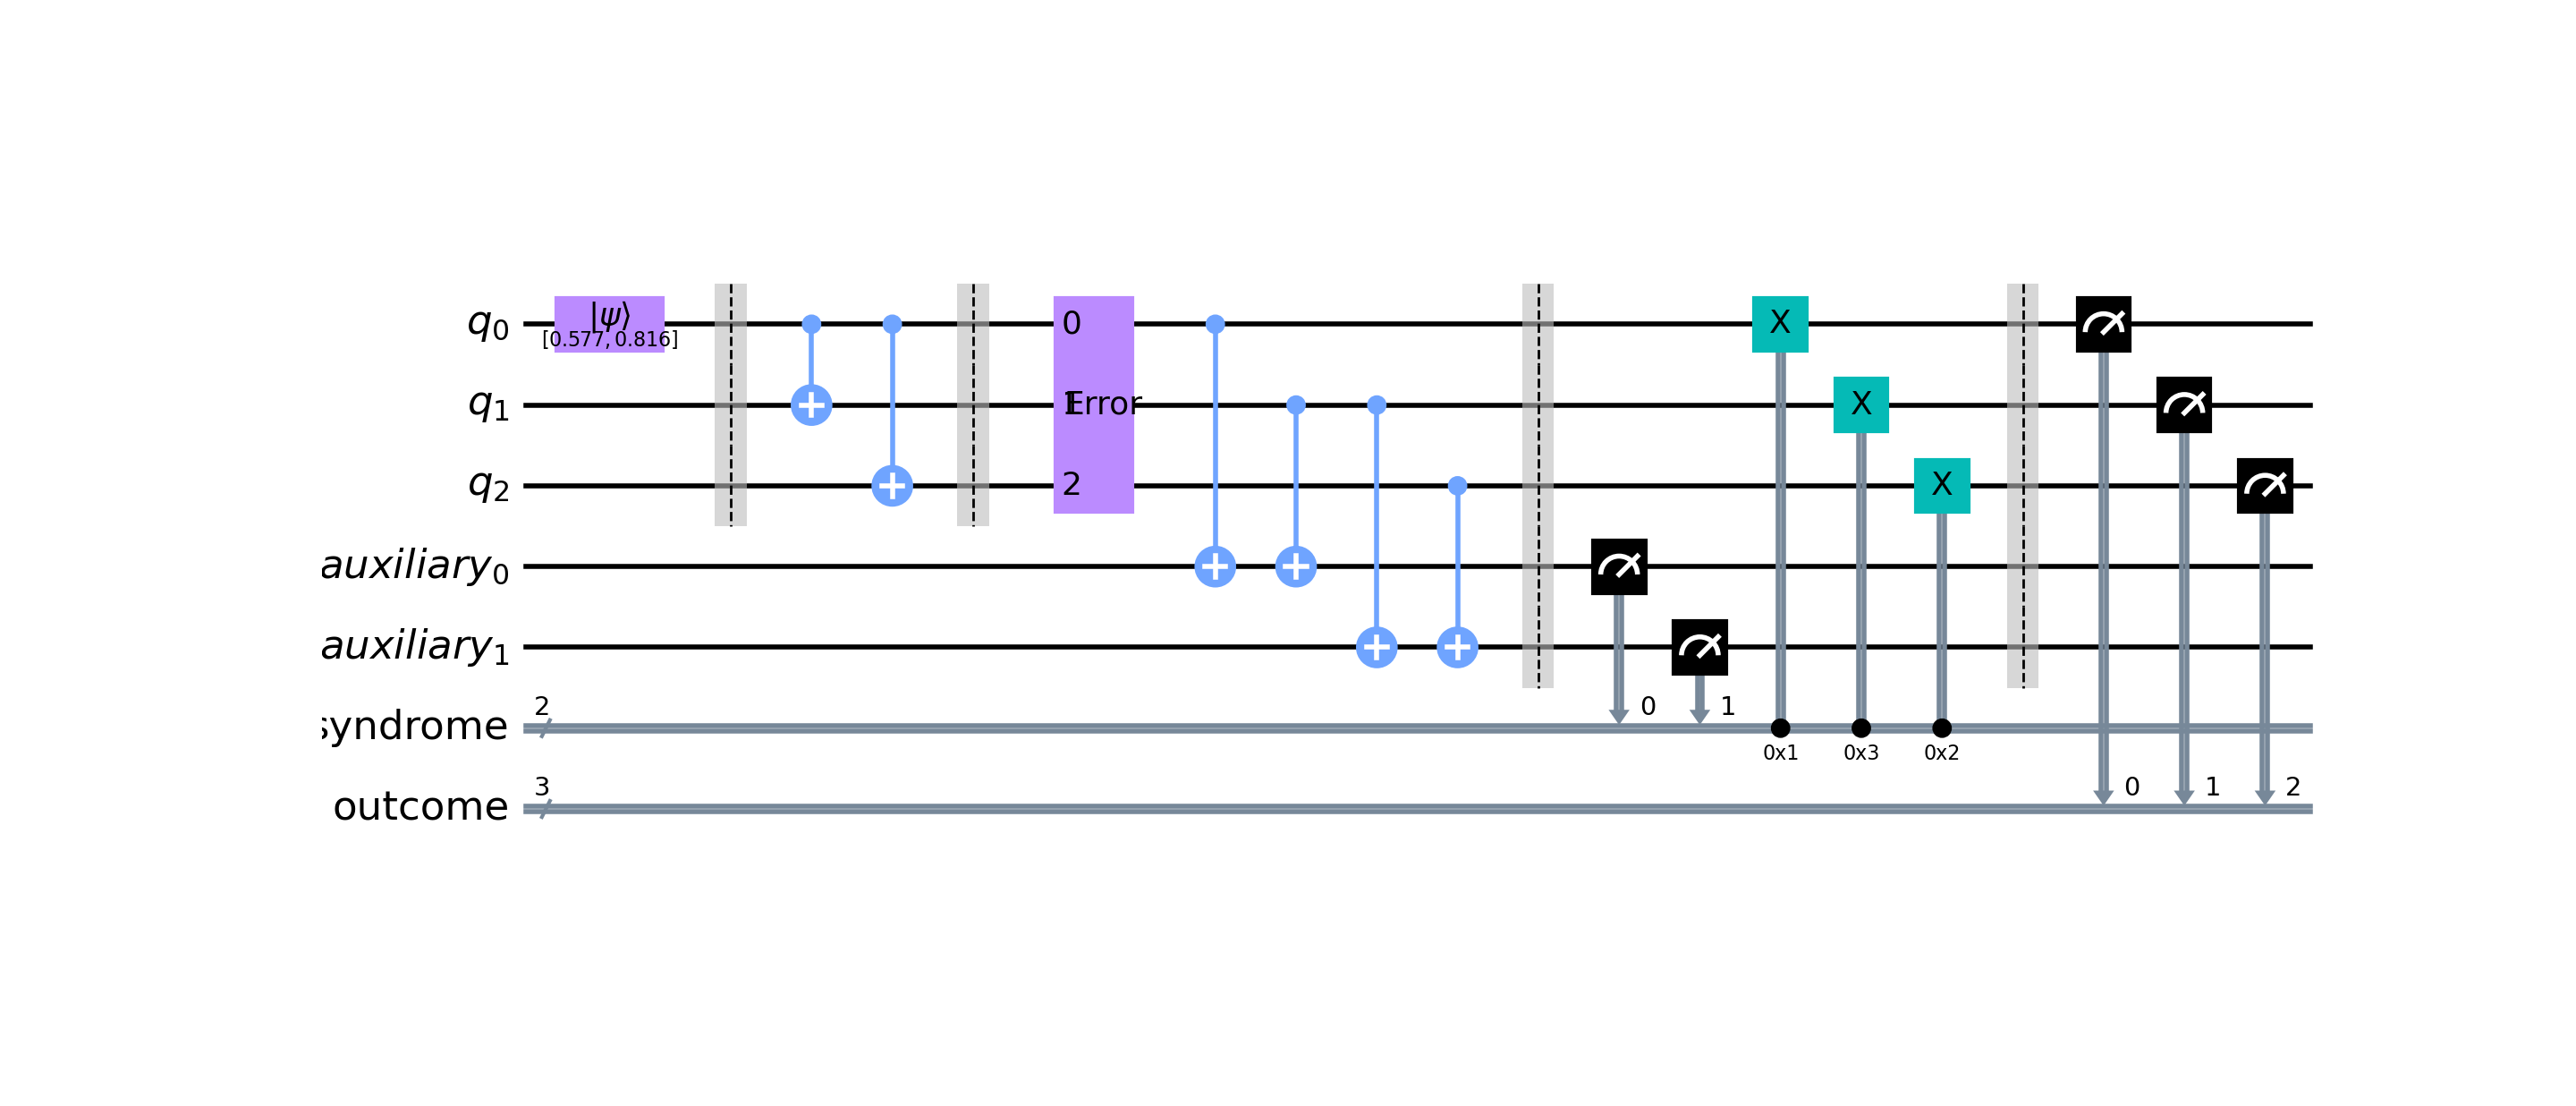
\includegraphics[width=\textwidth]{Mainmatter/images/3bitflipcode.png}
    \caption{Circuit for the 3 bit-flip error correction code, built with CNOT gates, which allows the correction of one X error on the encoded state. The M in the square represent a measurement on the ancilla qubits}
    \label{fig:3fq}
\end{figure}

The original information that we want to protect can be written without loss of generality as $\ket{\psi} = \alpha\ket{0}+\beta\ket{1}$.
As said in the previous section one might be tempted to clone the information like in the classical binary repetition code, but the no-cloning theorem prevents us from applying an operation that maps $\ket{\psi} \to \ket{\psi}\ket{\psi}\ket{\psi}$, showing that the classical idea cannot be directly taken over.
Instead, we can encode our qubit with other two qubits initially in the state $\ket{0}$. First we map the state $\ket{\psi} \to  \alpha\ket{000}+\beta\ket{100}$, then we apply two CNOT gates as shown in figure \ref{fig:3fq}, and encode the qubits in the following way: 
\begin{equation*}
  \alpha\ket{000}+\beta\ket{100} \to \alpha\ket{000}+\beta\ket{111} := \ket{\psi}_L
\end{equation*}
where we use the subscript $L$ to denote that the final encoded state lives in the logical two-dimensional subspace spanned by $\{\ket{0}_L = \ket{000} , \ket{1}_L = \ket{111}\}$ basis:
$$
|\psi\rangle_{L} \in \mathcal{C}=\operatorname{span}\{|000\rangle,|111\rangle\} \subset \mathcal{S}_{8}
$$
where $\mathcal{C}$ is called the codespace and its elements are the codewords.% We can also write the density operator that describe the system: $\rho=\ket{\psi_L}\bra{\psi_L}$.



Then the logical state $\ket{\psi}_L$ is sent down to the channel, and an error can occur. 


Notice that three individual bit flips are required to take $\ket{0}_L \leftrightarrow \ket{1}_L$, hence if we assume $\ket{\psi} = \ket{0}_L$, a single bit-flip on any qubit leaves the final state closer to $\ket{0}_L$ than $\ket{1}_L$. The distance between two codeword states, d, defines the number of errors that can be corrected, t, as, $t=\floor{\frac{d-1}{2}}$. In this case,d=3 because it is characterized by a weight $|\Tilde{X}|=|X_1 \otimes X_2 \otimes X_3 | = 3$ , hence $t=1$, but we will give a more in-depth explanation for the code distance and the number of correctable errors.



%The noise action on the qubits can be thought of as a set of Kraus operators which multiply the state of the system with some probabilities. We define an error set for the bit-flip noise: $\mathcal{E}=\left\{I,X^1,X^2,X^3\right\}$ as a set of operators proportional to Kraus operators. 
%The bit-flip noise acting on the qubit (i) can be written as: 
%\begin{equation*}
 %   \mathcal{E}^i(\rho) = (1-p)\rho +p X^i \rho X^i 
%\end{equation*}
%Generally, at least one of these operators (usually $\left.E_{0}\right)$ is taken to be the identity $I$ (at least to a good approximation), which corresponds to no error occurring, while the others represent possible errors. 
%Since the noise acts independently on each of the 3 qubits: 
%\begin{equation*}
 %   \mathcal{E}_{noise}(\rho)=\mathcal{E}^3(\mathcal{E}^2(\mathcal{E}^1(\rho)))
%\end{equation*} 
After the noisy channel the outcome state is one of the following:
\begin{equation*}
\begin{array}{ll}
\text { State } & \text { probability} \\
\alpha|000\rangle+\beta|111\rangle & (1-p)^{3} \\
\alpha|100\rangle+\beta|011\rangle & p(1-p)^{2} \\
\alpha|010\rangle+\beta|101\rangle & p(1-p)^{2} \\
\alpha|001\rangle+\beta|110\rangle & p(1-p)^{2} \\
% a|110\rangle+b|001\rangle & p^{2}(1-p) \\
% a|101\rangle+b|010\rangle & p^{2}(1-p) \\
% a|011\rangle+b|100\rangle & p^{2}(1-p) \\
% a|111\rangle+b|000\rangle & p^{3}
\end{array}
\end{equation*}
We get restricted on the case where only one physical qubit has been flipped, and ignore all the errors that flipped 2 or more qubits; in fact, the probability for this is of higher order $O(p^2)$ and the code will not be able to correct all of them.


Classically, single bit-flip errors are corrected by measuring the three bits and taking a majority vote. Here, this is not possible, since measuring the bits would project the system into one of the basis states with probability $|\alpha|^{2}$ or $|\beta|^{2}$,
destroying the superposition state that we are trying to protect. 

There is a two stage error-correction procedure which can be used to recover the correct quantum state without loosing the information: detect the error and correct it.  


In order to detect the error we have to do a measurement that reveals the error without revealing any information about the encoded state.
Error detection measurements are called syndrome measurements and the outcomes are called syndromes. 

In the quantum 3 bit-flip code one possible way to detect the error is to measure the correlation between two qubits, using two are commuting observables $Z_1 Z_2$ and $Z_2 Z_3$ with eigenvalues $\pm 1$.

%All four states are mutually orthogonal, hence they lie in orthogonal subspaces. Therefore, there is a quantum measurement that will tell which of these four subspaces the state is in without projecting onto a basis state and thereby destroying the superposition.

%We find that the outcomes of these syndrome measurements can detect and distinguish all single-qubit bit-flips, which can then be corrected. 


As shown in figure \ref{fig:3fq} this involves the use of two more qubits, these are called ancilla qubits.

The basic idea is to extract the syndrome performing two parity checks with the commuting observables $Z_1 Z_2$ and $Z_2 Z_3$ on the data block, and store the information in the ancilla qubits. 

Two initialized ancilla are then coupled to the data block as shown in figure \ref{fig:3fq}, using CNOT gates. 
We are left with 4 scenarios: 
\begin{equation*}
    \begin{array}{cc}
         \text{Error Location }& \text{Final State}, |data\rangle|ancilla\rangle \\
         \text{No Error} & (\alpha|000\rangle+\beta|111\rangle)|00\rangle \\
\text{Qubit 1} & (\alpha|100\rangle+\beta|011\rangle)|10\rangle \\
\text{Qubit 2} & (\alpha|010\rangle+\beta|101\rangle)|11\rangle \\
\text{Qubit 3} & (\alpha|001\rangle+\beta|110\rangle)|01\rangle 
    \end{array}
\end{equation*}
These ancilla are then measured. The measurement results indicate where (or if) an error has occurred, without directly measuring any of the data qubits.

In the end we use the value of the error syndrome to tell what procedure to use to recover the initial state:
\begin{equation*}
    \begin{array}{ccc}
        \text{Syndrome measurement:}
        (Z_1Z_2,Z_2Z_3) & \text{Ancilla state}& \text{Correction}\\
         (+1,+1) & |00\rangle & \text{Clean state, no correction needed }\\
(-1,+1) & |10\rangle & \text{Bit flip on qubit 1} \\
(-1,-1) & |11\rangle & \text{Bit flip on qubit 2}\\
(+1,-1) & |01\rangle  & \text{Bit flip on qubit 3}
    \end{array}
\end{equation*}

This bit-flip code has a correctable error set with four error operators: $\left\{I, X_{1}, X_{2}, X_{3}\right\}$. However, the full error set of this error model contained eight error operators. The three errors of weight- 2 and one error of weight-3 are uncorrectable errors. They produce states in the same four sub-spaces above, and it is easy to see that in the case of those high-weight errors the correction procedure will produce the erroneous state $\left|\psi_{L}^{\prime}\right\rangle=\alpha|111\rangle+\beta|000\rangle .$ In fact, the weight- 3 error will not even be recognized as an error: it is an undetectable error. This is a general property of QECCs: no QECC can correct every possible error. (This is also true of classical errorcorrecting codes.) In practice, the goal is to choose a code that can correct the most likely errors.

In analogous way of thinking, we can implement also the phase flip error code. In fact, a phase flip error in the computational basis ($\ket{0},\ket{1}$) can be seen as a bit flip in a new set of basis ($\ket{+},\ket{-}$), as shown in section \ref{sec:qgate}.

This suggests using the states $\ket{+},\ket{-}$ to create the logical encoded qubits: 
\begin{equation*}
    \begin{array}{c}
         \ket{0}_L=\ket{+++} \\
          \ket{1}_L=\ket{---}
    \end{array}
\end{equation*} these are the zero and the one states for protection against phase flip errors. 
To change basis in quantum circuit we can apply an Hadamard gate at appropriate points in the procedure.
The 3 phase-flip circuit is shown in figure \ref{fig:3phfc}

Then all the operations needed for error-correction are performed just as for the bit flip channel, but with respect to the new basis $\ket{+},\ket{-}$


We can improve our error analysis calculating the fidelity of this quantum error correction code, giving a measure of how reliable is this code against specific type of errors.
To calculate the fidelity is better to use the density matrix formalism, recalling the fact that the fidelity between a pure and a mixed state is given by :$ \mathcal{F}(\ket{\psi},\rho) = \bra{\psi}\rho\ket{\psi}$.
The object of quantum error-correction is to increase the fidelity with which quantum information is stored (or communicated) up near the maximum possible fidelity of one. Let’s compare the minimum fidelity achieved by the three qubit bit flip code with the fidelity when no error-correction is performed.
Suppose the quantum state of interest is $\ket{\psi}$ .
Without using the error-correcting code the state of the qubit after being sent through the channel is: 
\begin{equation*}
    \rho = (1-p)\ket{\psi}\bra{\psi} + p X\ket{\psi}\bra{\psi}X
\end{equation*}
Then the fidelity is given by
$$
F=\langle\psi|\rho| \psi\rangle=(1-p)+p\langle\psi|X| \psi\rangle\langle\psi|X| \psi\rangle
$$
The second term under the square root is non-negative, and equal to zero when $|\psi\rangle=|0\rangle$, so we see that the minimum fidelity is $F=1-p$ (No error correction code apply). Suppose the three qubit error correcting code is used to protect the state $|\psi\rangle=a\left|0_{L}\right\rangle+b\left|1_{L}\right\rangle.$ The quantum state after both the noise and error-correction is:
$$
\rho=\left[(1-p)^{3}+3 p(1-p)^{2}\right]|\psi\rangle\langle\psi|
$$
The omitted terms represent contributions from bit flips on two or three qubits. All the omitted terms are positive operators, so the fidelity we calculate will be a lower bound on the true fidelity. We see that $F=\langle\psi|\rho| \psi\rangle \geq (1-p)^{3}+3 p(1-p)^{2}$. That is, the fidelity is at least $1-3 p^{2}+2 p^{3}$, so the fidelity of storage for the quantum state is improved provided $p<1 / 2$.


\begin{figure}[h!]
    \centering
    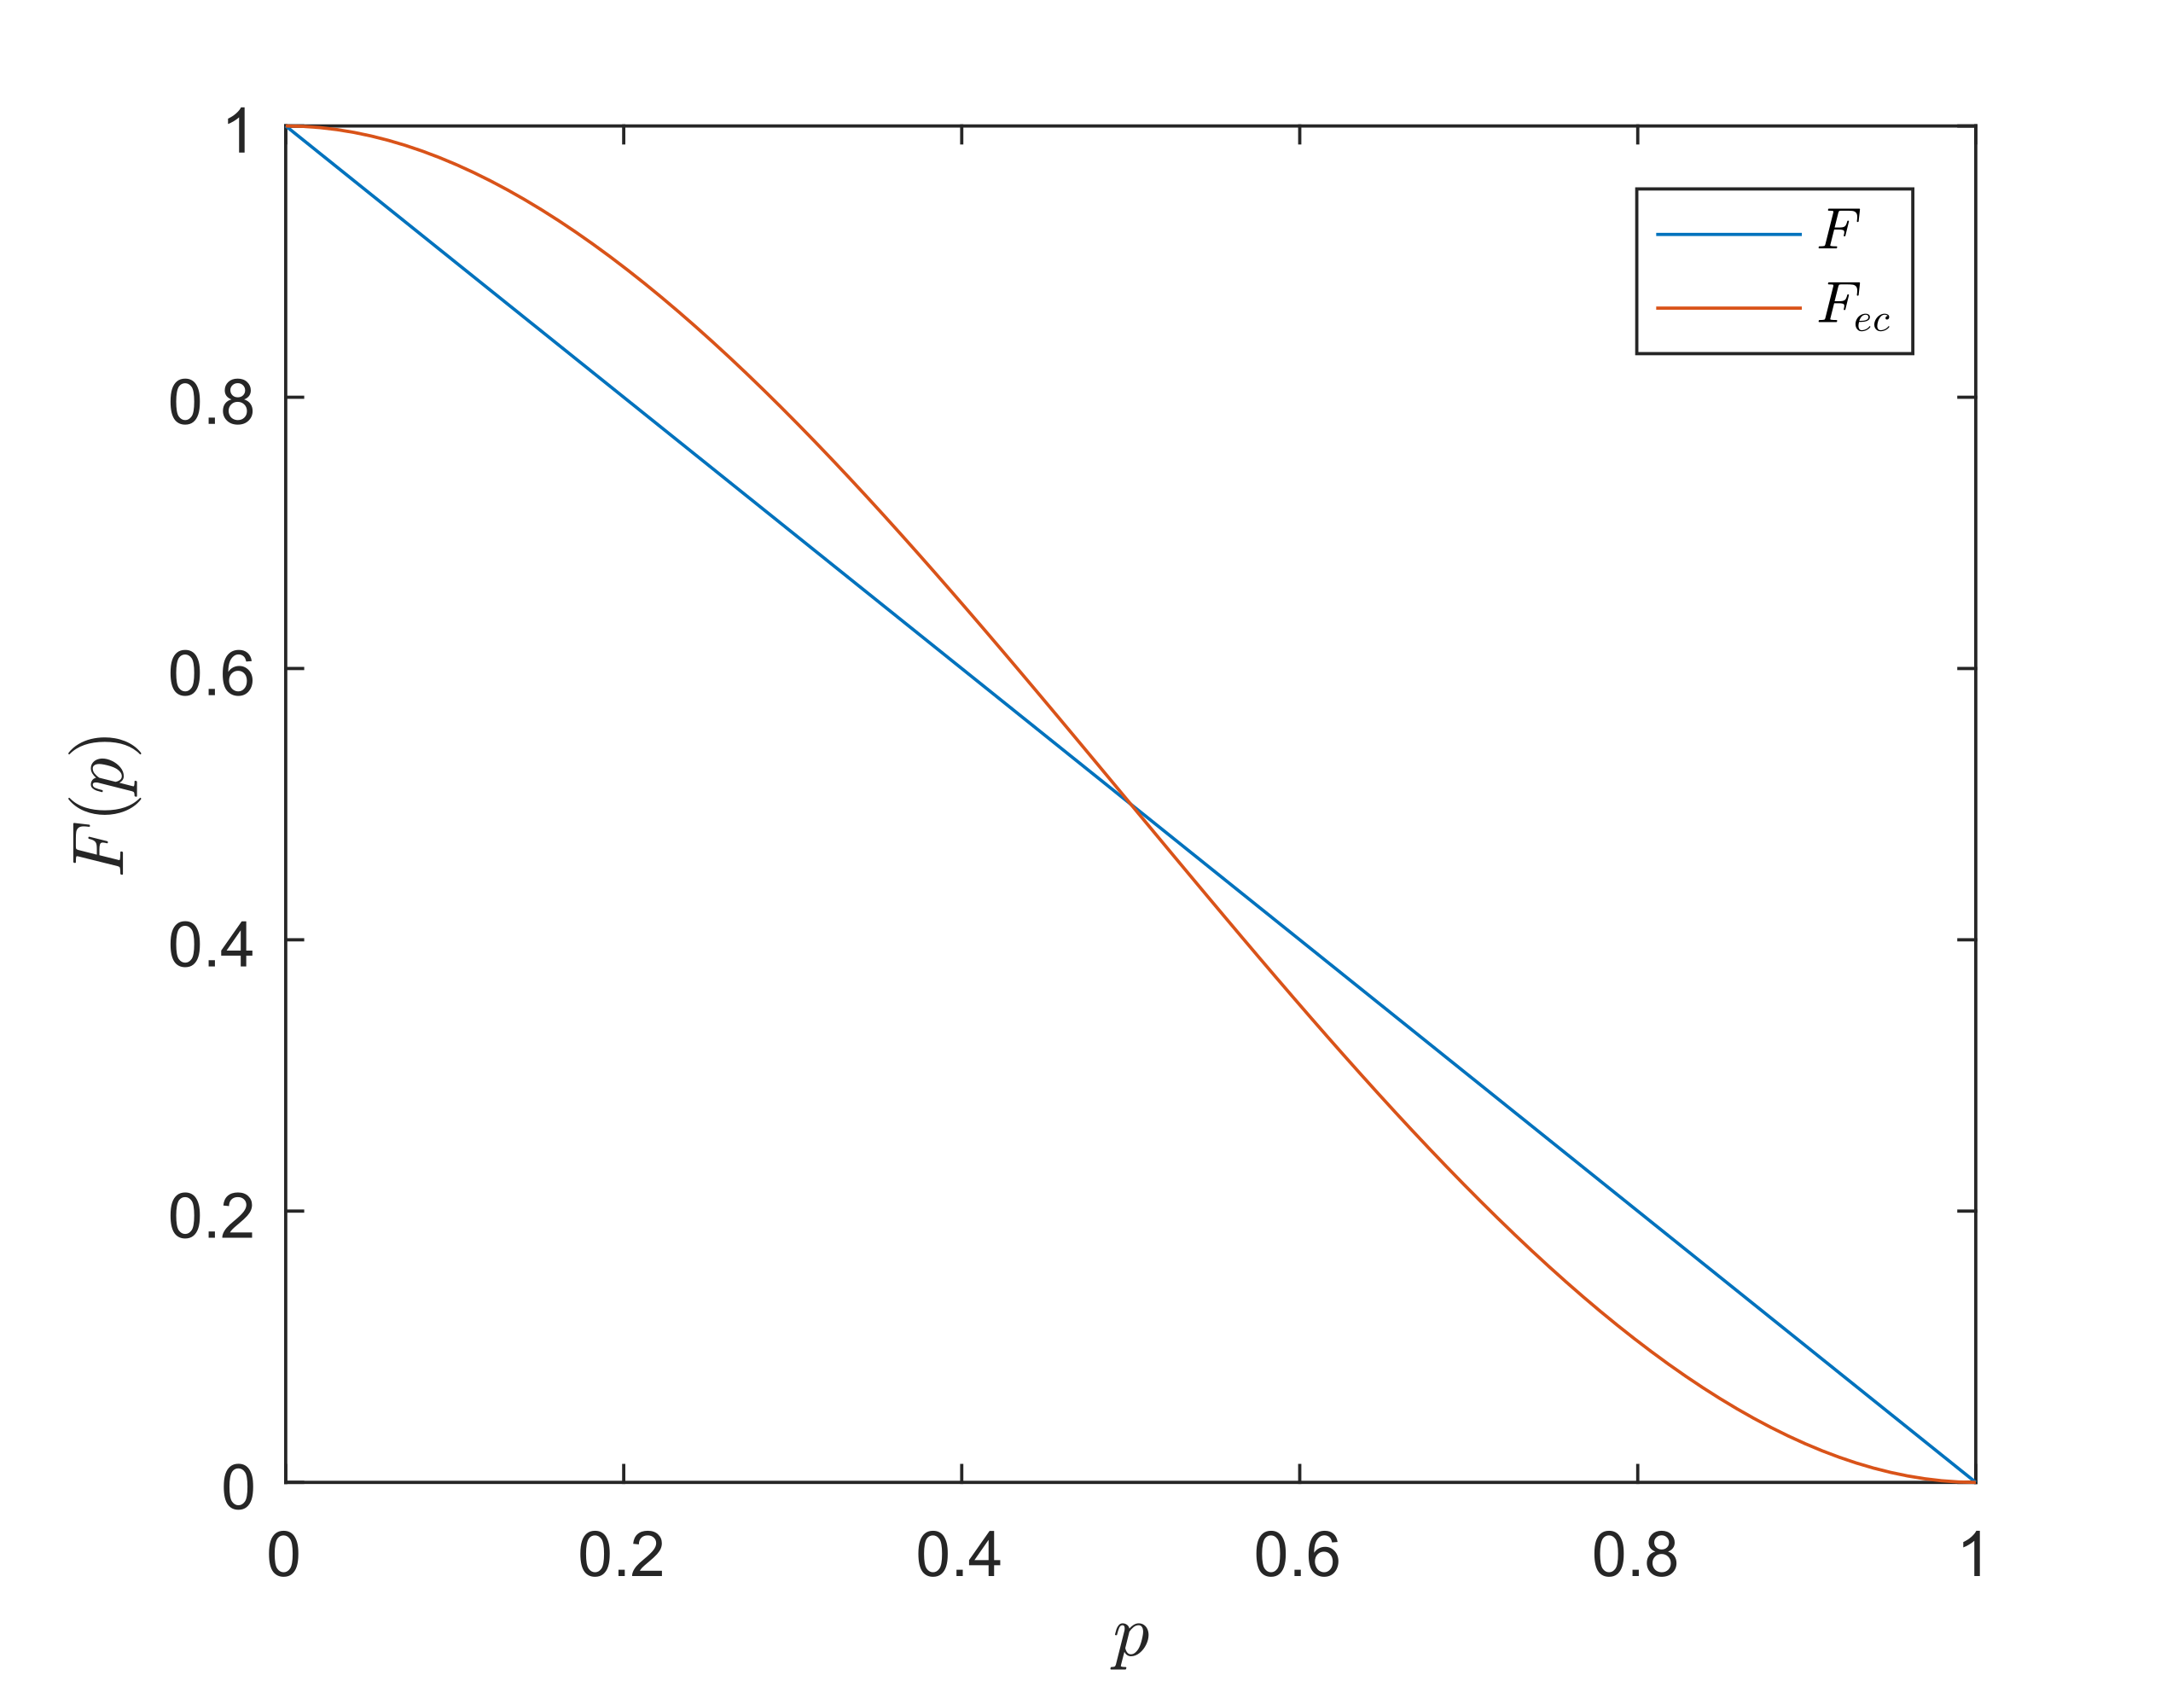
\includegraphics[scale=0.07]{Mainmatter/images/fidelity.png}
    \caption{In red the fidelity with the error correction procedure, in blue the fidelity without ( Currently this image is from wikipedia, but i will replace it with mine once I will do the computational part)}
    \label{fig:fidelity3qbit}
\end{figure}

\section{Stabilizer formalism}
In quantum error correction codes the description of quantum states becomes a difficult task when the number of qubits start rising, all the possible quantum states where the information can be projected by the noise grow exponentially in the number of qubits ($2^n$, where $n$ is the number of physical qubits). To understand complex quantum systems, it is essential to have efficient tools. The stabilizer formalism is a powerful tool that allows us to make general rules to construct preparation circuits, correction circuits and fault-tolerant logical gate operations once the stabilizer structure of the code is specified.


For example, the three-qubits code works by de-localising the information. The resultant logical state is then encoded in a two-dimensional subspace (the codespace $\mathcal{C}$) of the expanded Hilbert space. Then if an X-error occurs, the logical state is rotated to an orthogonal error space, an event that can be detected via a sequence of two stabilizer measurements and the result saved on some ancilla qubits, in the case of the three-qubit code the generators of the stabilizer group were $\{Z_1 Z_2 I, I Z_2 Z_3 \}$. 
%More in general the stabilizer formalism use the following scheme: 


%Usually a code is identified with this notation $[[n, k, d]]$ stabilizer codes, where $n$ is the total number of qubits, $k$ is the number of logical qubits and $d$ is the code distance. For instance the the three-qubit has $[[3,1,3]]$

%The advantage of entanglement-assisted stabilizer codes is that the sender can exploit the error-correcting properties of an arbitrary set of Pauli operators.

The definition of a stabilizer code is: 

Consider $\mathcal{S}=\{M\}$ to be a set of commuting error operators ($[M_i,M_j]=0 \quad \forall i,j$), this set is called Abelian. Since the operators all commute, they  have simultaneous eigenstates.
Let $\mathcal{C}=\{|u\rangle\}$ be an orthonormal set of simultaneous eigenstates all having eigenvalue $+1$:
\begin{equation}
M|u\rangle=|u\rangle \quad \forall u \in \mathcal{C}, \quad \forall M \in \mathcal{S}
\label{eq:stab}
\end{equation}
The set $\mathcal{C}$ is called codespace and its elements $|u\rangle$ are called code vectors or quantum codewords. 
A general state in the codespace is an encoded state or logical state, and it can be expressed as a superposition of the code vectors:
$$
|\psi\rangle_{L}=\sum_{u \in \mathcal{C}} a_{u}|u\rangle
$$ 
%Furthermore, $\mathcal{C}$ has $2^{k}$ members, since its members span a $2^{k}$ dimensional subspace of the $2^{n}$ dimensional Hilbert space of the whole system.
%On the other side, $\mathcal{S}$ is its stabilizer, its size is $2^{m}$, and it is spanned by $m =n-k$ linearly independent members of $\mathcal{S}$, where $n$ is the number of physical qubits and $k$ is the number of logical or encoded qubits.

%At this stage, the data previously stored solely in $\ket{\psi}$ is distributed across the expanded Hilbert space. 
A suitable stabilizer set of commuting operators acting on a single qubit can be a subgroup of the Pauli group:
$$
\mathcal{P}=\left\{\pm I, \pm i I, \pm X, \pm i X, \pm Y, \pm i Y, \pm Z, \pm i Z\right\}
$$

This set of matrices forms a group under the operation of matrix multiplication. The reason that the multiplicative factor $\pm 1 $ and $\pm i$ are included is to ensure that $\mathcal{P}$ is closed under multiplication, and thus forms a legitimate group. 
We can also generalize the concept of stabilizers for a system of multiple qubits. 
Given $n$ qubits a stabilizer set is a subgroup of the Pauli group $\mathcal{P}_n$, which is created by taking the $n$-fold tensor product of $\mathcal{P}$, i.e.
$$
\begin{aligned}
\mathcal{P}_{n} =\mathcal{P}^{\otimes n}
=\left\{\pm I, \pm i I, \pm X, \pm i X, \pm Y, \pm i Y, \pm Z, \pm i Z\right\}^{\otimes n}
\end{aligned}
$$

We can now define stabilizers more precisely: a subgroup $\mathcal{S} \subseteq \mathcal{P}_{n}$ is called stabilizer group of a system of $n$ qubits with $k$ logical qubits, and $\mathcal{C}$ is the vector space stabilized by $\mathcal{S}$.  

One feature of the stabilizer codes is that we can start from a stabilizer set and then deduct a codeword.
A perfect example, (again), is the three-qubit code ($n=3$), then start defining a stabilizer set $\mathcal{S} \equiv \{III,Z_1Z_2I,$ $IZ_2Z_3,Z_1IZ_3\}$. 
The subspace fixed by the operator $Z_1Z_2I$ is spanned by $|000\rangle$, $|001\rangle,|110\rangle$ and $|111\rangle$, and the subspace fixed by $IZ_{2} Z_{3}$ is spanned by $|000\rangle,|100\rangle,|011\rangle$ and $|111\rangle$. 
Note that the elements $|000\rangle$ and $|111\rangle$ are common to both these lists. Consequently, $\mathcal{C}$ must be the sub-space spanned by the states $|000\rangle$ and $|111\rangle$. 
Looking at this example we noticed that the sub-spaces have been stabilized by only two of the operators in $\mathcal{S}$.
In fact, mathematically a group can be described by its generators.
A set of elements $\{g1,...,gl\}$ in a group $G$ is said to generate the group $G$ if every element of $G$ can be written as a product of some of its elements. In the example $\mathcal{S}= \langle Z_1Z_2I,IZ_2Z_3\rangle$ as $Z_1IZ_3 = (Z_1Z_2I)(IZ_2Z_3)$ and $III = (Z_1Z_2I)^2$.
The great advantage of using generators to describe groups is that they provide a compact means of describing the group.
Nevertheless, not just any subgroup $\mathcal{S}$ of the Pauli group can be used as the stabilizer for a nontrivial vector space. For example, consider the subgroup of $\mathcal{P}_{1}$ consisting of $\{\pm I, \pm X\}$, the only solution to $(-I)|\psi\rangle=|\psi\rangle$ is $|\psi\rangle=0$, and thus $\{\pm I, \pm X\}$ is the stabilizer for the vector space with only the null vector. Hence, Two conditions are necessary in order not to span a trivial vector space :
\begin{enumerate}
    \item the stabilizer subgroup is Abelian ( i.e the elements of $\mathcal{S}$ commute)
    \item $-I$ and $-iI$ are not an element of the stabilizer set.
\end{enumerate}  

The definitions of stabilizer group and the codespace are of principal interest in QEC. 
One can show that if a stabilizer group $\mathcal{S}$ has $n-k$ independent generators, then $\operatorname{dim}[\mathcal{S}]=2^{n-k}$ and $\operatorname{dim}\left[\mathcal{C}\right]=2^{k}$, where $n$ indicates the number of physical qubits utilized and $k$ the logical qubits represented. %citare il libro
Whenever possible, $\mathcal{S}$ is typically represented through its independent generators $\mathcal{S}=<g_{1}, g_{2}, \ldots, g_{n-k}>$.





To understand how stabilizer codes detect and correct errors it is helpful to assume that the set of errors also consists of operators from the Pauli group. 

Each code allows correction of a particular set $\mathcal{E}=\{E\}$ of correctable errors.

Suppose that an error operator $E$ (which is also an element of the Pauli group) acts on the state. It anticommutes with some of the stabilizer generators, and commutes with others.
\begin{equation}
    M(E\ket{\psi}_L) = \pm EM\ket{\psi}_L = \pm (E\ket{\psi}_L)
    \label{eq:stabcond}
\end{equation}

Multiplying by $E$ changes the codeword to a new eigenstate of the stabilizer generators, where the eigenvalue is still $+1$ for all the generators that commute with $E$, but is $-1$ for those generators that anticommute with $E$.

%The eigenvalue of an operator $M$ from the stabilizer set detects errors which anticommute with $M$.
%On the contrary, if 
The measured eigenvalues $\lambda=\pm 1$ for each generator are the error syndrome.
To extract the syndrome we measure all the observables in the stabilizer. To do this, it is sufficient to measure any set of $n-k$ linearly independent $M$ in $\mathcal{S}$. Note that such a measurement has no effect on a state in the encoded subspace, since it is already an eigenstate of all these observables. The measurement projects a noisy state onto an eigenstate of each $M$, with eigenvalue $\lambda=\pm 1$.
The error can be deduced from the syndrome, hence to detect which error affected our logical qubit we need to store the results from the syndrome measurements. 

The syndrome extraction can be done most simply by attaching an $n-k$ qubit ancilla $A$ to the system, and storing in it the eigenvalues by a sequence of CNOT gates and Hadamard rotations.

The eigenvalue extraction of operator $M$, is done by preparing an ancilla in $(|0\rangle+|1\rangle) / \sqrt{2}$. 
Then, operate controlled-$M$ with ancilla as control, and system as target, then apply an Hadamard rotations to the ancilla. 
The final state of the ancilla is:  $[(1+\lambda)|0\rangle+(1-\lambda)|1\rangle] / 2$. In other words, if the stabilizer commute with the error operation ($\lambda=+1$) the ancilla final state will be $\ket{0}$, and viceversa. The syndrome measurements given by the application of the stabilizers are stored in the ancilla states. Repeating this process for all the $n-k$ operators $M$ which span $\mathcal{S}$, the effect is to couple system with the ancilla as follow:
$$
|0\rangle_{a} \sum_{i}\left(E_{i}|\phi\rangle_{L}\right) \rightarrow \sum_{i}\left|s_{i}\right\rangle_{a}\left(E_{i}|\phi\rangle_{L}\right)
$$
The syndromes $s_{i}$ are $(n-k)$ -bit binary strings. So far the treatment is completely general.
Now suppose the $E_{i}$ all have different syndromes. Then a projective measurement of the ancilla will collapse the sum to a single term taken at random: $\left|s_{i}\right\rangle_{a}\left(E_{i}|\phi\rangle_{L}\right)$, and will yield $s_{i}$ as the measurement result. 
The measurement result of the ancilla determines which eigenstate $\ket{\psi}_L$ is projected into.
Since there is only one $E_{i}$ with this syndrome, we can deduce the operator $E_{i}$ and correct it. 

This is the general prescription for correcting errors with a stabilizer code. One measures the values ±1 of the stabilizer generators; from the resulting error syndrome, one deduces which error occurred, and correct it(which for Pauli operators means just applying the error again). If the true error operator was actually a linear combination of Pauli operators, measuring the stabilizer generators will project the state into a joint eigenspace, and one proceeds exactly as if the error had been a Pauli operator. Just like linear codes, for a small stabilizer code one can use a look-up table of error syndromes; for a larger code, a decoding algorithm is needed.
% The exact network is shown in figure \ref{fig:stab}
% \begin{figure}[h!]
%     \centering
%     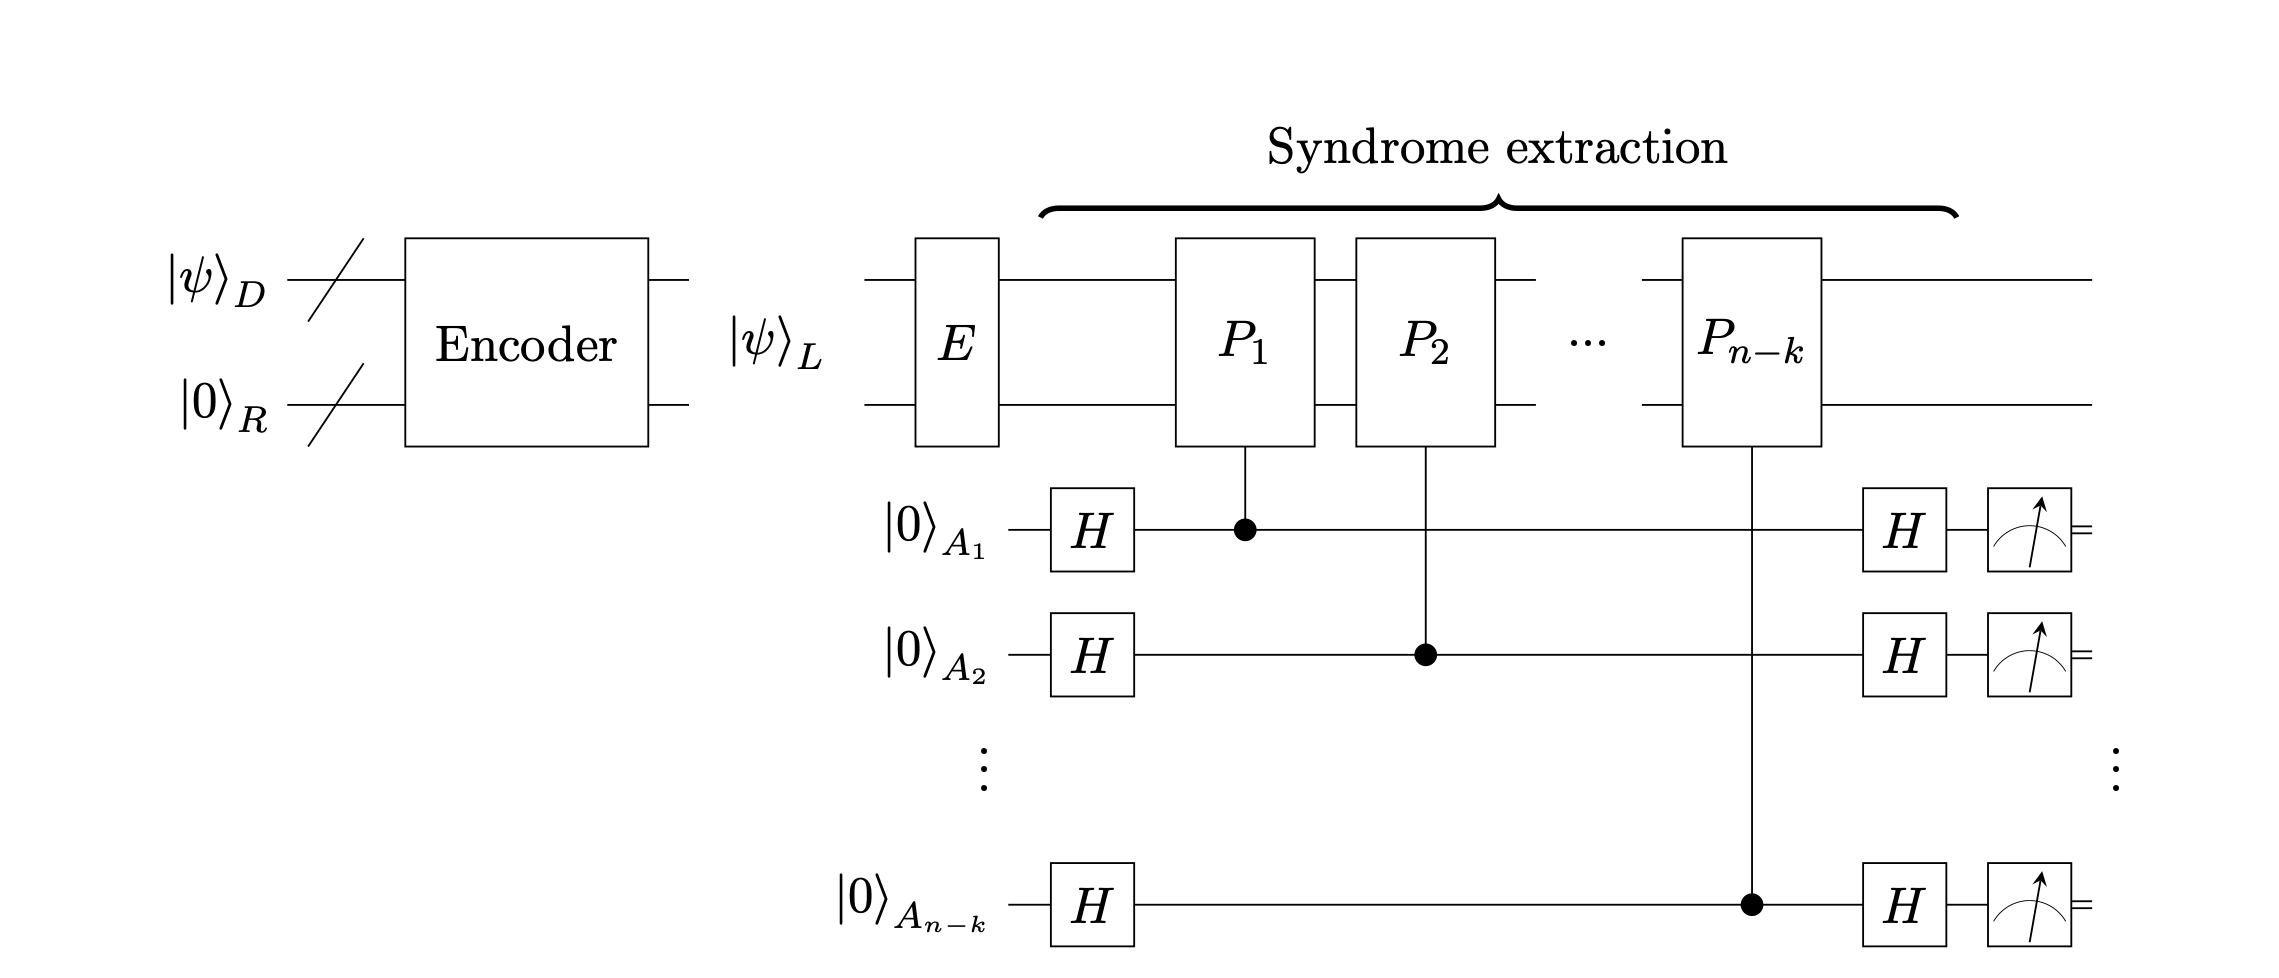
\includegraphics[width=\textwidth]{Mainmatter/images/Sindromeextraction.png}
%     \caption{}
%     \label{fig:stab}
% \end{figure}


Let us see how this works for the bit-flip code. It has generators $g_{1}=Z Z I$ and $g_{2}=I Z Z$. The three weight-one errors are $E_{1}=X I I, E_{2}=I X I, E_{3}=I I X .$ We can see that $E_{1}$ anticommutes with $g_{1}$ and commutes with $g_{2} ; E_{2}$ anticommutes with both $g_{1}$ and $g_{2}$; and $E_{3}$ anticommutes with $g_{2}$ and commutes with $g_{1}$. Since $g_{1}$ and $g_{2}$ are commuting observables, we can measure them to diagnose which error happened (or no error). The measured values $\pm 1$ for each generator are the error syndrome. Since Pauli operators are unitary and square to the identity, we can then undo the effects of the error by applying the appropriate Pauli operator again.

\section{Quantum code distance}
A quantum correction code can be identified by 3 parameters using the following notation: $[[n, k, d]]$\footnote{The doublebrackets are used simply to denote that the code being referred to is a quantum error correction code rather than a classical code.}. This means that a QECC encodes $k$ logical qubits using $n$ physical qubits , in such a way that any operation which maps some encoded state to another encoded state must act on at least $d$ qubits. 
So far we saw the physical and encoded qubits, but we never focused on the third parameter, so let's define what it is the code distance better, using the stabilizer formalism. 
As shown in the previous chapters, the eigenvalue of an operator $M \in \mathcal{S}$ from the stabilizer detects errors which anticommute with $M$.
On the other hand, if any of those errors which commute with $M$ occurs, the code it is not be able to detects the error anymore. This is because if we measure the eigenvalue of all the generators of the stabilizer they are all still $+1$, and also the correct codeword has eigenvalue $+1$ so there is no way that we can tell if any error occurs. In fact, stabilizer maps codewords in codewords, it is not that we don't measure the right thing actually there is no way to tell. 

In particular let's define a stabilizer set $\mathcal{S}$, and let $\mathrm{T}(\mathrm{S})$ be the corresponding QECC.
Define then,
$$
N(S)=\left\{N \in P_{n} \text { s.t. } M N=N M \forall M \in S\right\}
$$
and errors in this space are undetectable errors. 
Hence, we can say that a general QECC detects any error not in $\mathrm{N}(\mathrm{S}) \backslash \mathrm{S}$ (i.e., errors which commute with the stabilizer are not detected). We need also to remove all the error in $S$ because "errors" in S leave all codewords fixed, so are not really errors (Degenerate QECC, like the Shor code)
In this way, we are left with all those errors which anticommute with some M and can be detected. Starting from this point we can define the distance d. 
The distance d of $\mathrm{T}(\mathrm{S})$ is the weight of the smallest Pauli operator $\mathrm{N}$ in $\mathrm{N}(\mathrm{S}) \backslash \mathrm{S}$.

Intuitively, this can be though as the number of qubit that we need to flip to obtain another codeword. In other words, as is the case for classical codes, the distance of a quantum code is defined as the minimum size error that will go undetected.

This definition of distance tells us not only which errors can be detected but also how many of them can we correct. 
We can tell how many errors the code corrects by looking at operators that commute with the stabilizer. 



We say that a QECC can correct t errors if the set of errors that allow the recovery (those errors not in $\mathrm{N}(\mathrm{S}) \backslash S$) of weight t or less, must satisfy the sufficient conditions for the code to be able to correct the error: 
\begin{equation*}
    \bra{i} E_a^{\dagger}E_b \ket{j} = C_{a,b}\delta_{ij}
\end{equation*}
where $E_a^{\dagger}E_b \notin \mathrm{N}(\mathrm{S}) \backslash S$, and the states $i$ and $j$ are codewords.
%by  $E$ and $F$ if either $E^{\dagger} F \in S$ (so $E$ and $F$ act the same on codewords), or if $\exists M \in S$ s.t. $\left\{M, E^{\dagger} F\right\}=0$, in which case measuring the operator $M$ distinguishes between $E$ and $F$.
%The code correct errors for which $E^{\dagger}F \notin N(S) \backslash S$ for all possible pairs of errors E and F. 

Therefore, to correct t errors, we should look to all these pairs $E_a^\dagger E_b$ that show up in the criterion. Each $E_{a,b}$ acts on t qubit (correspondingly to the weight), but $E_a^\dagger E_b$ acts on $2t$ qubits. Then, the smallest thing in $N(S)\backslash S$ should be at least of weight $2t +1$. 


To sum up, if we want to correct error with  weight t, we need a code distance $d \ge 2t+1$.
Let's take a fast example, (again), the bit-flip code. 
In this code the smallest operator that transform $\ket{0}_L$ to $\ket{1}_L$, or vice versa, it
is $\Bar{X}=X_1X_2X_3$. 
If it were the case that qubits were only susceptible to $X-errors$, then the three-qubit code would have distance $d = 3$, cause each pauli operator has weight $1$
and to obtain another codeword you need 3 of them. 
However, as qubits are also susceptible to phase-flip errors like Z errors. The action of Z maps a codeword to another one, hence, for the bit-flip code a Z error is undetectable. Hence the real distance for this code is $d=1$. 
% In other words, this minimum size error can be viewed as a logical Pauli operator that transforms one codeword state to another. 



% This new eigenstate will always be orthogonal to the original codeword unless the error operator commutes with all the stabilizer generators.
%(So, for example, any encoded state which has been subjected to an error consisting of at most $\lfloor(d-1) / 2\rfloor$ Pauli operations can in principle be recovered perfectly).
%This notation generalises the notation $[n, k, d]$ for classical error correction codes. %in such a way that at least $d$ bits must be flipped to transform between any two codewords representing different plaintexts. (In this context and in the quantum case, $d$ is referred to as the code distance.) 
%
%The distance is the smallest size of a detectable error




\section{Shor code, $[[9,1,3]]$}
The Shor code is an example of a distance-three degenerate code for which it is possible to apply a successful recovery operation for any single-qubit error. This code uses 9-qubits, and it was the first QECCs that was capable of correcting any arbitrary error (Phase and bit flip) on a single qubit, protecting one logical qubit state.
The Shor code can be constructed by concatenating the bit-flip code and the phase-flip code. 
Code concatenation involves embedding the output of one code into the input of another.
So let's start building the encoded Shor states from the codespace of the bit-flip and the phase-flip code. 

Consider the codespace of a single bit-flip code: 
$$
\mathcal{C}_{3b}=\operatorname{span}\left\{|0\rangle_{3b}=|000\rangle,|1\rangle_{3 b}=|111\rangle\right\}, \quad \mathcal{S}_{3 b}=\left\langle Z_{1} Z_{2}, Z_{2} Z_{3}\right\rangle
$$
where $\mathcal{S}_{3b}$ are the code stabilizers. Similarly, codespace for phase-flips $\mathcal{C}_{3 \mathrm{p}}$ is defined
$$
\mathcal{C}_{3 \mathrm{p}}=\operatorname{span}\left\{|0\rangle_{3 \mathrm{p}}=|+++\rangle,|1\rangle_{3 \mathrm{p}}=|---\rangle\right\}, \quad \mathcal{S}_{3 \mathrm{p}}=\left\langle X_{1} X_{2}, X_{2} X_{3}\right\rangle
$$
Then to build the nine-qubit code, the bit-flip code is embedded into the codewords of the phase-flip code. This concatenation maps the $|0\rangle_{3 \mathrm{p}}$ codeword of the phase-flip code to a nine-qubit codeword $|0\rangle_{9}$ as follows
$$
|0\rangle_{3 \mathrm{p}}=|+++\rangle \stackrel{\text { concatenation }}{\longrightarrow}|0\rangle_{9}=|+\rangle_{3 \mathrm{b}}|+\rangle_{3 \mathrm{b}}|+\rangle_{3 \mathrm{b}}
$$
where $|+\rangle_{3 \mathrm{~b}}=\frac{1}{\sqrt{2}}(|000\rangle+|111\rangle)$ is a logical state of the bit-flip code. 

Similarly, the concatenation maps the $|1\rangle_{3 \mathrm{p}}$ codeword of the phase-flip code to
$$
|1\rangle_{3 \mathrm{p}}=|---\rangle \stackrel{\text { concatenation }}{\longrightarrow}|1\rangle_{9}=|-\rangle_{3 \mathrm{~b}}|-\rangle_{3 \mathrm{~b}}|-\rangle_{3 \mathrm{~b}},
$$
where $|-\rangle_{3b}=\frac{1}{\sqrt{\Omega}}(|000\rangle-|111\rangle)$. The code defined by the codewords $|0\rangle_{9}$ and $|1\rangle_{9}$ is the nine-qubit Shor code with paramaters $[[9, 1, 3]]$


Finally, the qubit state (the sending information) $|\psi\rangle=\alpha|0\rangle+\beta|1\rangle$ is encoded as $\left|\psi_{L}\right\rangle=\alpha\left|0_{L}\right\rangle+\beta\left|1_{L}\right\rangle$. Hence the codespace basis is: 
\begin{equation*}
\begin{split}
\left|0_{L}\right\rangle=\frac{1}{2 \sqrt{2}}(|000\rangle +|111\rangle) \otimes(|000\rangle +|111\rangle) \otimes(|000\rangle +|111\rangle) \\
\left|1_{L}\right\rangle=\frac{1}{2 \sqrt{2}}(|000\rangle -|111\rangle) \otimes(|000\rangle -|111\rangle) \otimes(|000\rangle -|111\rangle) 
\end{split}
\end{equation*}

Once one has find the codespace, it can also can look for a stabilizer set. Since this code is a concatenation of the bit-flip code and the phase-flip code one might use the same stabilizers but with more accuracy. 
A suitable stabilizer set is spanned by: 
\begin{equation}
\begin{aligned}
\mathcal{S}_{[[9,3,3]]}=&\left\langle Z_{1} Z_{2}, Z_{2} Z_{3}, Z_{4} Z_{5}, Z_{5} Z_{6}, Z_{7} Z_{8}, Z_{8} Z_{9}\right.\\
&\left.X_{1} X_{2} X_{3} X_{4} X_{5} X_{6}, X_{4} X_{5} X_{6} X_{7} X_{8} X_{9}\right\rangle
\end{aligned}
\end{equation}

The first six terms are the stabilizers of the bit-flip codes in the three-blocks of the code. The final two stabilizers derive from the stabilizers of the phase-flip code.

Hence, using the stabiliser formalism we can proceed for the syndrome measurement. 
\begin{table}[h]
    \centering
    \begin{tabular}{cc|cc}
\hline Error & Syndrome, $S$ & Error & Syndrome, $S$ \\
\hline$X_{1}$ & 10000000 & $Z_{1}$ & 00000010 \\
$X_{2}$ & 11000000 & $Z_{2}$ & 00000010 \\
$X_{3}$ & 01000000 & $Z_{3}$ & 00000010 \\
$X_{4}$ & 00100000 & $Z_{4}$ & 00000011 \\
$X_{5}$ & 00110000 & $Z_{5}$ & 00000011 \\
$X_{6}$ & 00010000 & $Z_{6}$ & 00000011 \\
$X_{7}$ & 00001000 & $Z_{7}$ & 00000001 \\
$X_{8}$ & 00001100 & $Z_{8}$ & 00000001 \\
$X_{9}$ & 00000100 & $Z_{9}$ & 00000001 \\
\hline
\end{tabular}
\caption{The syndrome table for single-qubit $X$ and $Z$ errors on the nine-qubit code. The nine-qubit code is a degenerate code, as certain $Z$ errors share the same syndrome}
    \label{tab:stab9}
\end{table}

Table \ref{tab:stab9} shows the syndromes for all single-qubit errors in the nine-qubit code. Each of the $X$ errors produce unique syndromes. In contrast, $Z$ -errors that occur in the same block of the code have the same syndrome. Fortunately, this degeneracy in the code syndromes does not reduce the code distance. To see why this is the case, consider the single-qubit errors $Z_{1}$ and $Z_{2}$, both of which map to the syndrome '00000010'. The decoder therefore has insufficient information to differentiate between the two errors, and will output the same recovery operation for either. For the purposes of this example, we will assume that the recovery operation the decoder outputs is $\mathcal{R}=Z_{1}$. For the case where the error is $E=Z_{1}$, the recovery operation restores the logical state as $\mathcal{R} E|\psi\rangle_{9}=Z_{1} Z_{1}|\psi\rangle_{9}=|\psi\rangle_{9} .$ In the event where $E=Z_{2}$, the recovery operation still restores the logical state as $\mathcal{R} E=Z_{1} Z_{2}$ is in the stabilizer of $\mathcal{C}_{[[9,1,3]]}$, and therefore acts on the logical state as follows $Z_{1} Z_{2}|\psi\rangle_{9}=|\psi\rangle_{9} .$ The same arguments can be applied to the remaining degenerate errors of the code. As a result, the nine-qubit code has the ability to correct all single-qubit errors and has distance $d=3$
In this code the process of correcting a X error or a Z error is totally independent: 
the inner layer of the code corrects bit flip errors taking the majority within each set of three, so 
On the other hand, the outer layer corrects phase flip errors: We take the majority of the three signs,
Since these two error correction steps are independent, the code also works if there is both a bit flip error and a phase flip error, and since $Y = iZX$, a $Y$ error can be thought as a single $X$ error and a single $Z$ error acting on the same qubit, up to an irrelevant global phase.

So this code can correct any Pauli error acting on a single qubit. However, even this is not the limit. Note that any operator on a single qubit can be written as a linear combination $E= aI + bX + cY+dZ$ for some complex numbers $a,b,c,d$. This allow us, using this code, to correct also a continuous tipe of errors. For instance, suppose the action of a general phase error on the codeword: 
$$
R_{\theta / 2}=\left(\begin{array}{cc}
1 & 0 \\
0 & e^{i \theta}
\end{array}\right)=e^{i \theta / 2}\left(\begin{array}{cc}
e^{-i \theta / 2} & 0 \\
0 & e^{i \theta / 2}
\end{array}\right)
$$
(with an overall phase that does not matter), we can write it as
$$
R_{\theta / 2}=\cos \frac{\theta}{2} I-i \sin \frac{\theta}{2} Z .
$$
It turns out that our earlier error correction procedure will also correct this error.
This can suggest a bigger result expressed by the following theorem [3]:

\begin{theorem}
If a quantum code corrects errors A and B, it also corrects any linear combination of A and B. In particular, if it corrects all weight t Pauli errors, then the code corrects all t-qubit errors.
\end{theorem}


\section{CSS codes}
CSS codes are a very special class of stabilizer codes with special properties. In fact, principles from the theory of classical error correction codes can be adapted for the construction of quantum error correction codes. Those quantum error correction codes can be driven from the classical codes and are called CSS codes.
Before introducing a CSS code construction, is better to do a brief recall of classical error correction codes, and we will take the Hamming code as a landmark.
There are two ways of representing a classical linear code and find its codewords: either as the image of a matrix G called the generator matrix or as the kernel of matrix H called the parity check matrix. More precisely we can define a linear classical error correcting code $\mathcal{C}$ of n-bit vectors by: $x \in \mathcal{C} \iff  Hx = 0$ with the linear property: $x,y \in \mathcal{C} \rightarrow x+y \in \mathcal{C}$. Moreover, $HG^T=0$ because each row of the generator matrix is a codeword and must satisfy the parity check; the other codewords are all linear combinations of the rows of the generator matrix.
%Another important definition is the dual code $\mathcal{C}^{\perp}$ of a linear code $\mathcal{C}$, this is the code whose generator matrix is the parity check matrix of $\mathcal{C}$. 
We can deduce a similarity between the parity check matrix and the stabilizer set. 
In fact, in classical codes if an error occur it affects the codeword as follow $x+e_1$ , and no longer satisfy the parity check $H(x+e_1) = He_1 \neq 0$. An analogous situation corresponds when an error occurs and the condition (\ref{}) is no longer satisfied.  
Hence, we can see the rows of H as indicators of which stabilizers are needed.
A well known classical correcting code is the Hamming code which is [7,4,3]. The parity check of this code is: 
\begin{equation*}
    H=\left(\begin{array}{ccccccc}
         1&1&1&1&0&0&0  \\
         1&1&0&0&1&1&0 \\
         1&0&1&0&1&0&1 
    \end{array}\right) 
\end{equation*}
If we replace each 1 in this matrix by the operator Z, and 0 by I, we are just specifying three operators that implement the parity check measurements. The statement that the classical Hamming code corrects one error is the statement that each bit flip error of weight one or two anticommutes with one of these three operators.
\begin{equation*}
    H_1=\left(\begin{array}{ccccccc}
         1&1&1&1&0&0&0  \\
         1&1&0&0&1&1&0 \\
         1&0&1&0&1&0&1 
    \end{array}\right) \to \mathcal{S}_{bf}=\left\langle\begin{array}{ccccccc}
         Z&Z&Z&Z&I&I&I  \\
         Z&Z&I&I&Z&Z&I \\
         Z&I&Z&I&Z&I&Z 
    \end{array}\right\rangle
\end{equation*}
However, qubits are subjected to phase-flips as well. We can use again the same procedure; we replace each 1 by X instead of Z and we can correct a phase error. We again get three operators, and they will anticommute with any weight one or two Z error.
\begin{equation*}
    H_2=\left(\begin{array}{ccccccc}
         1&1&1&1&0&0&0  \\
         1&1&0&0&1&1&0 \\
         1&0&1&0&1&0&1 
    \end{array}\right) \to \mathcal{S}_{pf}=\left\langle\begin{array}{ccccccc}
         X&X&X&X&I&I&I  \\
         X&X&I&I&X&X&I \\
         X&I&X&I&X&I&X 
    \end{array}\right\rangle
\end{equation*}
Thus, if we make a stabilizer out of the three Z operators and the three X operators, we get a code that can correct any single qubit error. X errors are picked up by the first three generators, Z errors by the last three, and Y errors are distinguished by showing up in both halves. 
\begin{equation}
    \mathcal{S} : \begin{array}{ccccccc}
         Z&Z&Z&Z&I&I&I  \\
         Z&Z&0&I&Z&Z&I \\
         Z&I&Z&I&Z&I&Z \\
         X&X&X&X&I&I&I  \\
         X&X&I&I&X&X&I \\
         X&I&X&I&X&I&X 
         \end{array}
         \label{eq:stabSteane}
\end{equation}
We solved a difficult problem as finding a stabilizer set of a quantum error correcting code with a minimum effort using the knowledge from the classical theory.
But there is one thing that we need to pay attention when we use this procedure: the stabilizer must be Abelian, i.e. all the elements commute.
In the previous example, the stabilizer set is Abelian and the corresponded code is the Steane code $[[7,1,3]]$.
 
This example uses the same classical code for both the $X$ and $Z$ generators, but there was no reason to do so. We could have used any two classical codes $C_{1}$ and $C_{2}$. The only requirement is that the $X$ and $Z$ generators commute. This corresponds to the statement that $C_{2}^{\perp} \subseteq C_{1}\left(C_{2}^{\perp}\right)$ is the dual code to $C_{2}$\footnote{$C_2^{\perp}$ is the dual code of $C_2$, intuitively this means that in $C_2^{\perp}$ the generator matrix and the parity matrix are switched respect $C_2$. In other words it consists  of those words which are orthogonal to the codewords of $C_{2}$)}.
If $C_{1}$ is an $\left[n, k_{1}, d_{1}\right]$ code, and $C_{2}$ is an $\left[n, k_{2}, d_{2}\right]$ code, then the corresponding quantum code is an $\left[\left[n, k_{1}+k_{2}-n, \min \left(d_{1}, d_{2}\right)\right]\right]$ code. 

   %have a particularly nice form. One way to write down the quantum codewords is:
% $$
% |u\rangle_{L}=\frac{1}{\sqrt{dim(C_2^{\perp})}}\sum_{x \in C_{2}^{\perp}}|x+u \cdot D\rangle
% $$
% where $u$ is a $k$ -bit binary word, $x$ is an $n$ -bit binary word, and $D$ is a $(k \times n)$ matrix of coset leaders. A coset leader is a word of minimum weight in any particular coset, which is a word with the lowest amount of non-zero entries We can understand the structure of these codewords as follows. 
% Start with the case $u=0: |0\rangle_{L}$ is an equal superposition of all the members of $C_{2}^{\perp}.$ 
% The next encoded state is found by displacing all the members of $C_{2}^{\perp}$ by the same vector (the first row of $\left.D\right)$ : in other words we have a superposition of all the members of a coset. We choose the vector (the coset leader) so that this coset is still in $C_{1}$. The other quantum codewords are formed similarly by further cosets of $C_{2}^{\perp}$, all within $C_{1}$. Bit flip correction follows from the%They all must satisfy the same parity checks as the classical code $C_{1}$, so all codewords will be superpositions of codewords of $C_{1} .$ The parity check matrix of $C_{2}$ is the generator matrix of $C_{2}^{\perp}$, so the $X$ generators of the stabilizer add a word of $C_{2}^{\perp}$ to the state. Thus, the codewords of a CSS code are of the form
% $$
% \sum_{w \in C_{2}^{\perp}}|u+w\rangle
% $$
% where $u \in C_{1}\left(C_{2}^{\perp} \subseteq C_{1}\right.$, so $\left.u+w \in C_{1}\right) .$

%The basis of the quantum code 
The codewords of a CSS code, in this case the Steane code, include two entangled states obtained from the classic codewords of each coset of $\mathrm{C}_1$ relative to $\mathrm{C}_2^{\perp}:$ the logical 0 is given from all the codewords with even weight $\mathrm{C}_2^{\perp} \oplus(0000000)$:
% and the $\mathrm{C}^{\perp} \oplus(1111111)=\{$ codewords of $\mathrm{C}$ with odd weight $\}$. The quantum codewords are:

$$
\begin{array}{r}
\left|0\right\rangle_L=\frac{1}{\sqrt{8}}[|0000000\rangle+|1010101\rangle+|0110011\rangle+|1100110\rangle \\
+|0001111\rangle+|1011010\rangle+|0111100\rangle+|1101001\rangle]
\end{array}
$$
To determine the other logical codeword we need to find an element of $C_{1}$ that is not in $C^{\perp}_{2}$. An example of such an element is $(1111111)$, giving then the other logical qubit, which this time is formed by all the codewords with odd weight:
$$
\begin{array}{r}
\left|1\right\rangle_L=\frac{1}{\sqrt{8}}[|1111111\rangle+|0101010\rangle+|1001100\rangle+|0011001\rangle \\
\quad+|1110000\rangle+|0100101\rangle+|1000011\rangle+|0010110\rangle]
\end{array}
$$

% Suppose that $C_{1}$ and $C_{2}$ are $[n,k_1,d_1]$ and $[n_2, k_2,d_2]$ two classical linear codes such that $C_2 \in C_i$ and $C_1$ and $C_2^{\perp}$ both correct t errors.
% So a CSS code of $C_{1}$ over $C_{2}$ as an $\left[n, k_{1}+k_{2}-n, d\right]$ code, with $d \geq 2 t+1$ and $d=min(d_1,d_2)$, and can be constructed as follow: 

% let $x$ be any codeword in $\in C_{1}.$ Then, we define a quantum state: 
% \begin{equation*}
%      \left|x+C_{2}\right\rangle:=\frac{1}{ \sqrt{\left|C_{2}\right|} }\sum_{y \in C_{2}}|x+y\rangle
% \end{equation*}where $+$ is the binary addition.
% Then $\operatorname{CSS}\left(C_{1}, C_{2}\right)$ is defined as $\left\{\left|x+C_{2}\right\rangle \mid x \in C_{1}\right\}$

\section{Quantum Hammming bound}
Even if CSS code construction is a very straightforward and elegant procedure, it not guarantees that we can create the best QECC code from classical codes. In fact, exists a better QECC with $[[5,1,3]]$. Can we do better than this? Actually no, there is an upper bound that we cannot cross over if we want to construct an error correction code. This bound is the hamming bound. 
Unfortunately the quantum Hamming bound only applies to non-degenerate codes, but it gives us an idea of what more general bounds may look like.

Suppose a non-degenerate code is used to encode $k$ qubits in $n$ qubits in such a way that it can correct errors on any subset of t or fewer qubits. Suppose $j$ errors occur, where $j\leq t$. There are $\left(\begin{array}{c}
     n\\
     j
\end{array}\right)$ set of locations where errors may occur. With each such set of locations there are three possible errors (the 3 pauli matrices X,Y,Z) that may occur on a single qubit for a total of $3^j$ possible errors. The total number of errors that may occur on $t$ or fewer qubits is therefore: 
\begin{equation*}
    \sum_{j=0}^t 3^j\left(\begin{array}{c}
     n\\
     j
\end{array}\right)
\end{equation*}
where $j=0$ corresponds to the case where there is no error. In order to encode $k$ qubits in a non-degenerate way each of these errors acting on each basis codeword produces a linearly independent state, must correspond to an orthogonal 2k-dimensional subspace. All these subspaces must be fit in the $2^n$-dimensional available to n qubits, leading to the inequality:
\begin{equation}
    \left(\sum_{j=0}^t 3^j\left(\begin{array}{c}
     n\\
     j
\end{array}\right)\right)2^k \leq 2^n
\label{Hamming}
\end{equation}
This relation is called the quantum Hamming bound. 
To understand the power of this relation consider, for example, the case where we wish to encode one qubit in n qubits in such a way that errors on one qubit are tolerated.
Substituting $t=1,k=1$ in \ref{Hamming}, we obtain the relation: 
\begin{equation*}
    2(1+3n)\leq2^n
\end{equation*}
This is satisfied only for $n\geq 5$. In fact, the $[[5,1,3]]$ is the best quantum error correction code. There is no code that encodes one qubit in fewer than five qubits in such a way as to protect from all possible errors on a single qubit.
A non-degenerative code for large $n$ and $t$, $R=\frac{k}{n}$ (Rate) fixed the best nondegenerate quantum codes satisfy: 
\begin{equation*}
    \frac{k}{n} \leq 1 - \frac{t}{n}log_2(3) - H(\frac{t}{n})
\end{equation*}
where H is the entropy function ($H(x)=-xlog_2(x) -(1-x)log_2(x)$)
\include{Mainmatter/Quantum_code_distance}
\chapter{Fault-Tolerant computation}
\section{Introduction to fault tolerant computation}
So far we had a sort of communication scenario where Alice wants to send information to Bob and the error occurs in the noisy channel. 
Then we developed good algorithms to contrast errors that happen in between, protecting the information.
To do that we supposed that Alice and Bob were dealing with perfect quantum computers with perfect gates and perfect operations. 
However, nature is far from this. 
The error can occur while we are doing any quantum operations, also during the quantum error correction procedure.
Noise afflicts each of the elements used to build this circuit : the state preparation procedures, quantum logic gates, measurement of the output, and even the simple transmission of quantum information along quantum wires.

To face this problem we can use fault-tolerant computation, which computes directly on encoded quantum states in such a manner that decoding is never required. Hence, each qubit in the original circuit is replaced with an encoded block of qubits, using an error-correcting code such as the seven qubit Steane code, and each gate in the original circuit is replaced with a procedure for performing an encoded gate acting on the encoded state. 
One might think performing error-correction periodically after every operation, but this is not sufficient to prevent the build-up of errors.
%Two are the reasons: first, the encoded gates can cause errors to propagate and second is that error-correction itself can introduce errors on the encoded qubits, so we must be careful to design error-correction procedures that do not introduce too many errors into the encoded data
%%%%%%%%%
%Aggiusta 
%%%%%%%%%%
% In fact, one of the most powerful applications of quantum error-correction is not merely the protection of stored or transmitted quantum information, but the protection of quantum information as it dynamically undergoes computation.
% Moreover, a fault-tolerant computation and protocols prevent from catastrophic events of error propagation by ensuring that a single faulty gate or time step produces only a single error in each block of quantum error correction codes. Hence, a fault tolerant computation is that the circuits used for gate operations and error correction procedures should not cause errors to cascade or propagate along the circuit.
%%%%%%%%%
%ERROR PROPAGATION
%%%%%%%%%

In fact, when we perform multiple qubits gates during a quantum computation, any existing error can propagate to other qubits, even if the gate itself can be considered perfect.
For instance, a CNOT gate can propagate forward (from control qubit to the target qubit) a bit-flip error. In figure \ref{fig:CNOT_prop} a bit-flip error occurs on the control qubit just before the CNOT gate.
This single error will cascade forward (from control to target) such that the X error propagates on both output qubits after the gate.

We started with 1 error and we ended up with 2 errors. 
\begin{figure}[h!]
    \centering
    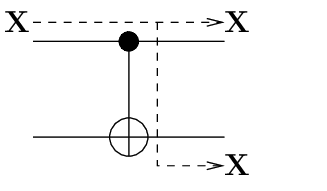
\includegraphics[scale=0.5]{Mainmatter/images/XCNOT.png}
    \caption{A CNOT gate can cause a X error to propagate forward so that instead of affecting one qubit, it affects two. This is also true when encoded qubits are used, and an encoded CNOT is implemented.}
    \label{fig:CNOT_prop}
\end{figure}

Another example, that has not any classical analogy, is the backwards (from target to control) propagation. Imagine having a CNOT and a Z error occurs just before on the target qubit, then after the CNOT we will have 2 phase errors on both qubits as shown in figure \ref{fig:CNOT_prop2} .

\begin{figure}[h!]
    \centering
    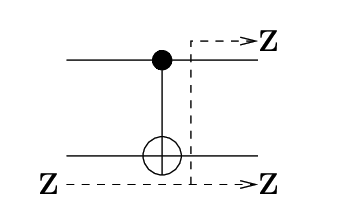
\includegraphics[scale=0.5]{Mainmatter/images/ZCNOT.png}
    \caption{A CNOT gate can cause a Z error to propagate backwards so that instead of affecting one qubit, it affects two. This is also true when encoded qubits are used, and an encoded CNOT is implemented.}
    \label{fig:CNOT_prop2}
\end{figure}
This is clearly a problem if we build an arbitrary circuit that implements CNOT gates and a QECC that corrects up to 1 error, it is not able to correct the propagated error anymore.
Thus, by error propagation, a correctable local error is converted into a non-correctable one. The procedure described is thus not fault tolerant.




Hence, to achieve a fault tolerant computation we first need to implement fault tolerant logic operations, which prevent the building up of errors in the same error correction block. A solution is to perform logic gates transversally - i.e. a transversal gate interacts the ith qubit in one block with the ith qubit of the other block. Recall single encoded qubit gates involving only one block are transversal, because the ith qubit interacts with itself.
For instance, in the Steane code the logical $\Bar{X}=X^{\otimes 7} $ and $\Bar{Z}=Z^{\otimes 7}$ operations on a single encoded
qubit are the first examples of valid transversal codeword operations.
% The spreading of single-qubit errors during imperfect gates to more than one qubit in the output can be prevented if the gates are implemented in a transversal manner. That is, the gates shall be implemented using only independent operations on each of the physical qubits. Logical gates that are implemented in this way are naturally fault-tolerant since any error on a single physical qubit can not propagate to another physical qubit in the encoded state.
For any stabilizer codes, a large class of operations can be performed on logical data in a fault-tolerant way. 
Furthermore, the performed operations must map codewords to codewords.



More precisely, if a given logical state, $|\psi\rangle_{L}$ is stabilized by $M \in \mathcal{S}$, and the logical operation $U$ is applied, the new state, $U|\psi\rangle_{L}$ is stabilized by $U M U^{\dagger} \in \mathcal{S}$, i.e,
\begin{equation}
(U M U^{\dagger}) U|\psi\rangle_{L}=U M|\psi\rangle_{L}=U|\psi\rangle_{L}
\end{equation}
Hence, for $U$ to preserve the codespace, $U M U^{\dagger}$ must be in the stabiliser set.
This properties is satisfied for any $U \in \mathbf{C}$ where $\mathbf{C}$ is called the Clifford group:
\begin{definition}
Let $\mathcal{P}_{n}$ be the Pauli group on $n$ qubits and let $\mathcal{U}\left(2^{n}\right)$ be the unitary group. The Clifford group $\mathbf{C}_{n}$ on $n$ qubits is,
\begin{equation}
\mathbf{C}_{n}=\left\{U \in \mathcal{U}\left(2^{n}\right): U P U^{\dagger} \in \mathcal{P}_{n} \text { for all } P \in \mathcal{P}_{n}\right\}
\end{equation}
The Clifford group on $n$ qubits can be generated by Hadamard gate $H, R_{\pi / 4}$ gate, and CNOT gate, where
$$
H=\frac{1}{2}\left(\begin{array}{cc}
1 & 1 \\
1 & -1
\end{array}\right), \quad R_{\pi / 4}=e^{-i \pi / 4}\left(\begin{array}{cc}
1 & 0 \\
0 & i
\end{array}\right), \quad \operatorname{CNOT}=\left(\begin{array}{cccc}
1 & 0 & 0 & 0 \\
0 & 1 & 0 & 0 \\
0 & 0 & 0 & 1 \\
0 & 0 & 1 & 0
\end{array}\right) .
$$
\end{definition}
From this we can notice also how error how errors change after applying quantum gates: 
the operation of $U$ on an erroneous codeword $E|\psi\rangle$ gives,
\begin{equation}
U E|\psi\rangle=\left(U E U^{\dagger}\right) U|\psi\rangle
\label{eq:spread}
\end{equation}
Observe that $U|\psi\rangle$ is a state from the operation of $U$ on state $|\psi\rangle$.
Here we can see that the error $E$ before the operation $U$ becomes $U E U^{\dagger}$ after the operation of $U$. 
So now our goal is to implement the generators of clifford group in a fault-tolerant way. Let us think this in the context of the seven qubit code $[[7,1,3]]$ with its stabiliser set (\ref{eq:stabSteane}). 

\subsection*{Fault-tolerant Hadamard and $R_{\pi/4}$}
A logical Hadamard gate $\bar{H}$ interchanges $\bar{Z}$ and $\bar{X}$ under conjugation, just as the Hadamard gate $H$ interchanges $Z$ and $X$ under conjugation. $\bar{H}= H^{\otimes 7}$ accomplishes this task, so that a Hadamard on the encoded qubit can be implemented as in figure \ref{fig:logHada}
\begin{figure}[h!]
    \centering
    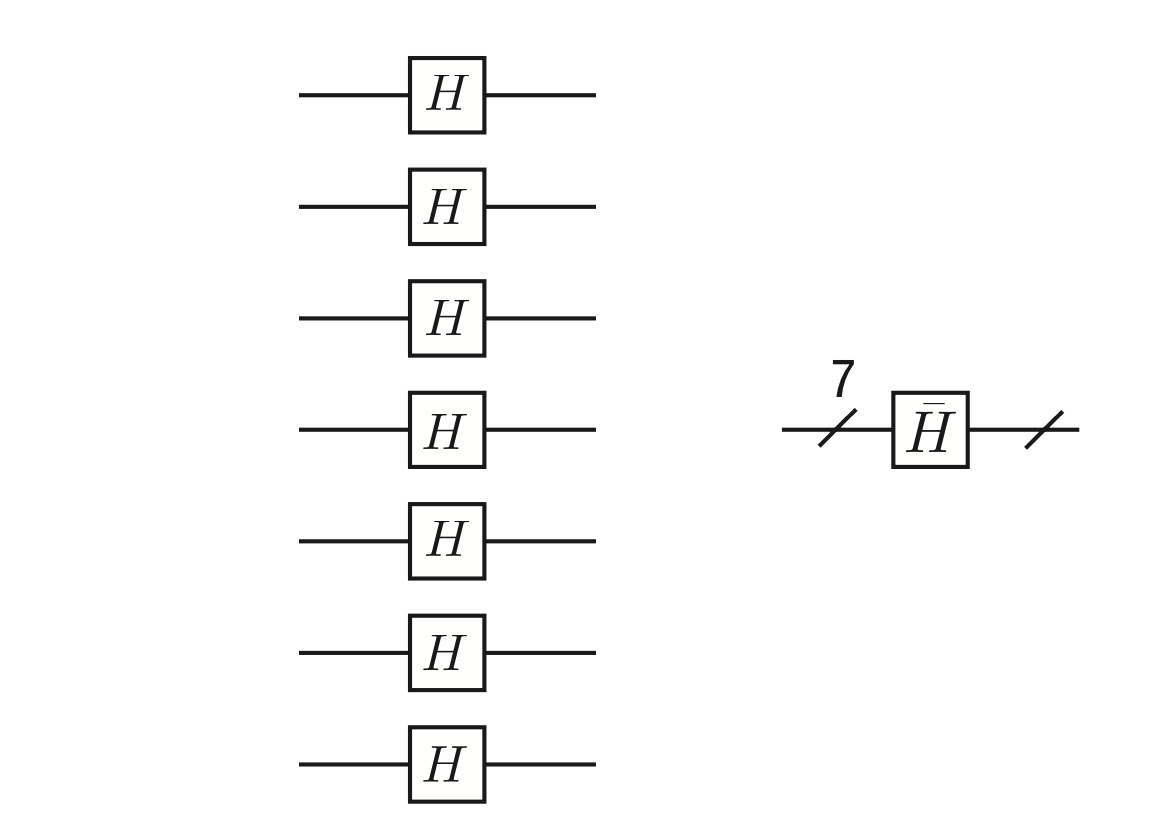
\includegraphics[scale=0.5]{Mainmatter/images/LogicalHadamard.png}
    \caption{This figure shows the logical hadamard gate. On the right is showed a more compact notation, the 7 and the slash on the wire indicate that we are operating on an encoded state}
    \label{fig:logHada}
\end{figure}

This is fautl-tolerant because the failure of a single component in the circuit can cause at most one error in the block of qubits output from the procedure. To see that this is true suppose that a $Z$ error occurs on the first qubit just before the encoded $H$ gate was applied. The combined operation on the qubit is $H Z$. Then, we can use the equation \ref{eq:spread}, which describes how an error spreads after applying a gate, hence it gives $H Z =(H Z H^{\dagger})H=X H$, so such an error is equivalent to first applying $H$ then the error $X$ occurring.

Moreover, $\Bar{H}$ maps stabilisers in other stabiliser, let us take the first stabilizer $M_1=ZZZZIII \in \mathcal{S}$ and we see that $\Bar{H} M_1 \Bar{H} = M_4 =XXXXIII $ which is still in the stabilizer. 

A very similar construction can be implemented also for the $\frac{\pi}{4}$ logical operation.  The $\frac{\pi}{4}$ rotation gate single qubit $R_{\pi/4}$ gate leaves $Z$ unaltered, while $X$ is mapped to $Y=iXZ$. However, applying 
$\Bar{R_{\pi/4}}=R_{\pi/4}^{\otimes7}$ takes $\bar{Z}$ to $\bar{Z}$ under conjugation, and $\bar{X}$ to $-\bar{Y}.$ The minus sign in front of the $-\bar{Y}$ may be fixed up by applying $\bar{Z}$.
Thus, applying the operation $Z R_{\pi/4}$ to each qubit in the code effects an encoded phase gate, which is transversal and thus fault-tolerant.


\subsection*{Fault-tolerant CNOT gate}

A two qubit logical CNOT operation can also be applied in the same transversal way. For un-encoded qubits, a CNOT operation performs the following mapping on the two qubit stabilizer set,
$$
\begin{array}{l}
X \otimes I \rightarrow X \otimes X \\
I \otimes Z \rightarrow Z \otimes Z \\
Z \otimes I \rightarrow Z \otimes I \\
I \otimes X \rightarrow I \otimes X .
\end{array}
$$
Where the first operator corresponds to the control qubit and the second operator corresponds to the target. This can be extended to the logical space, we can apply the logical CNOT operation between two encoded states: 
$$
\begin{array}{l}
\bar{X} \otimes I \rightarrow \bar{X} \otimes \bar{X}, \\
I \otimes \bar{Z} \rightarrow \bar{Z} \otimes \bar{Z}, \\
\bar{Z} \otimes I \rightarrow \bar{Z} \otimes I, \\
I \otimes \bar{X} \rightarrow I \otimes \bar{X} .
\end{array}
$$
The issue of Fault-tolerance with these logical operations should be clear. The $\bar{X}, \bar{Z}, \bar{H}$ and $\bar{R}_{\frac{\pi}{4}}$ gates are fault-tolerant since the logical operation is performed through seven single qubit gates. The logical CNOT is also fault-tolerant since each two-qubit gate only operates between counterpart qubits in each logical block as shown in figure \ref{fig:TransCNOT} . Hence if any gate is inaccurate, then at most a single error will be introduced in each block, and we are able to correct 1 error per block. 
\begin{figure}[h!]
    \centering
    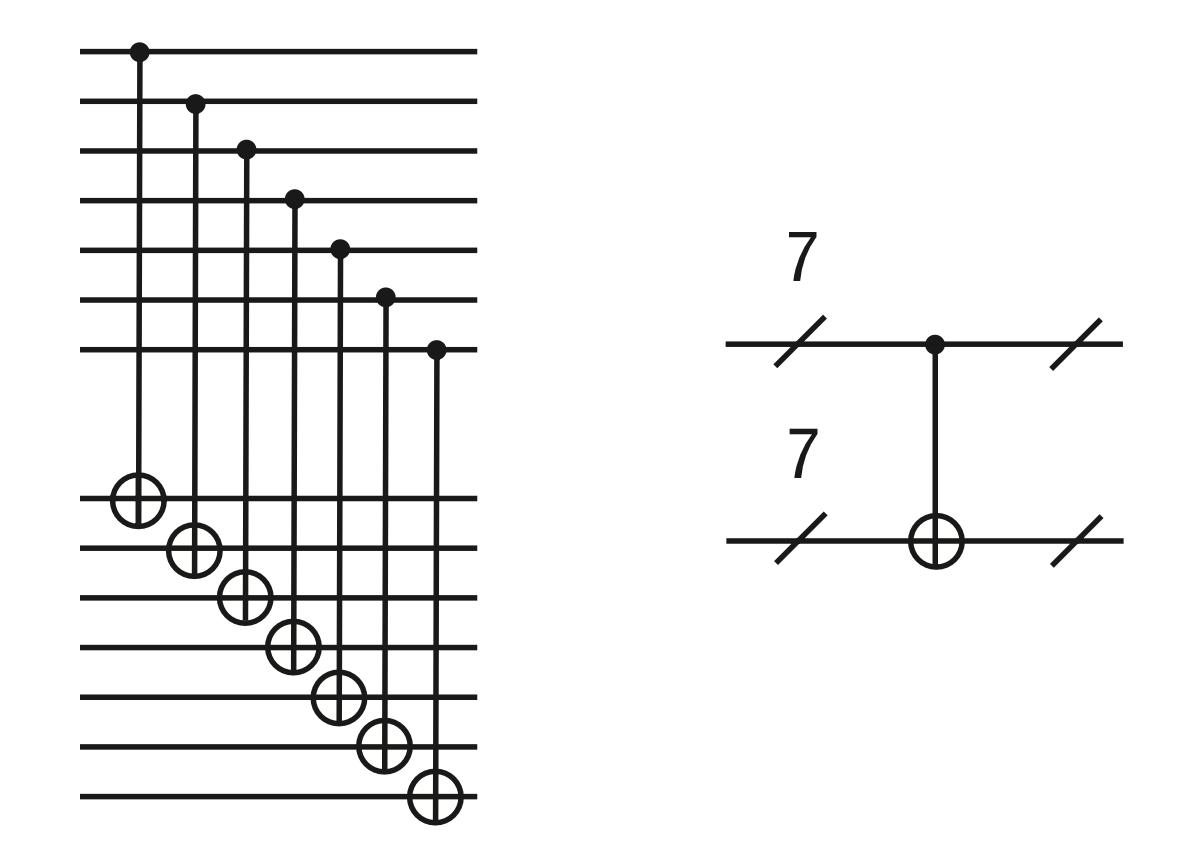
\includegraphics[scale=0.5]{Mainmatter/images/Transversal_CNOT.png}
    \caption{This figure shows a transversal fault-tolerant CNOT between two encoded qubits.}
    \label{fig:TransCNOT}
\end{figure}
A fault-tolerant CNOT is also a good example to show that the error probability goes from $p$ to $cp^2$.
%Might add that probability of 1 error goes from p to p^2
% In contrast to the $[[7,1,3]]$ code, let us also take a quick look at the $[[5,1,3]]$ code. The $[[5,1,3]]$ code is a non-CSS code, the Clifford group of gates cannot be fully implemented in transversal manner. To see this clearly we can examine how the stabilizer group for the code transforms under transversal Hadamard operation:
% $$
% \left(\begin{array}{ccccc}
% X & Z & Z & X & I \\
% I & X & Z & Z & X \\
% X & I & X & Z & Z \\
% Z & X & I & X & Z
% \end{array}\right) \quad \longrightarrow\left(\begin{array}{ccccc}
% Z & X & X & Z & I \\
% I & Z & X & X & Z \\
% Z & I & Z & X & X \\
% X & Z & I & Z & X
% \end{array}\right)
% $$
% The stabilizer group is not preserved under this transformation, therefore the transversal Hadamard operation is not valid for the $[[5,1,3]]$ code. One thing to briefly note that there is a method for performing logical Hadamar and phase gates on the $[[5,1,3]]$.

Nevertheless, the Clifford group is not an universal set of operation.  
The Gottesman-Knill theorem states that if a quantum circuit consists of only these elementary operations, the operation of the circuit can be efficiently simulated by a classical computer \cite{gottesman1998heisenberg}. This means that if we want to construct a quantum computer that fully exploits the power of quantum computation, only aforementioned operations are not sufficient.

In order to achieve universality one of the following gates are generally added to the available set: $R_{\pi/8}$ or the Toffoli gate. 
Although both gates can be implemented in a fault-tolerant way through a more complicate procedure called "Magic state injection", in the following it will focus only the fault-tolerant implementation of  $R_{\pi/8}$ gate. 

The basic idea of this procedure is based on the concept of teleportation, which is briefly described in the appendix.
Let us begin by not worrying about fault-tolerance, and simply attempt to perform some gate $\bar{U}$ on an encoded state. 
We will consider the case of a single-qubit gate $\Bar{U}$ first. \cite{gottesman2009introduction}

\begin{figure}[h!]
    \centering
    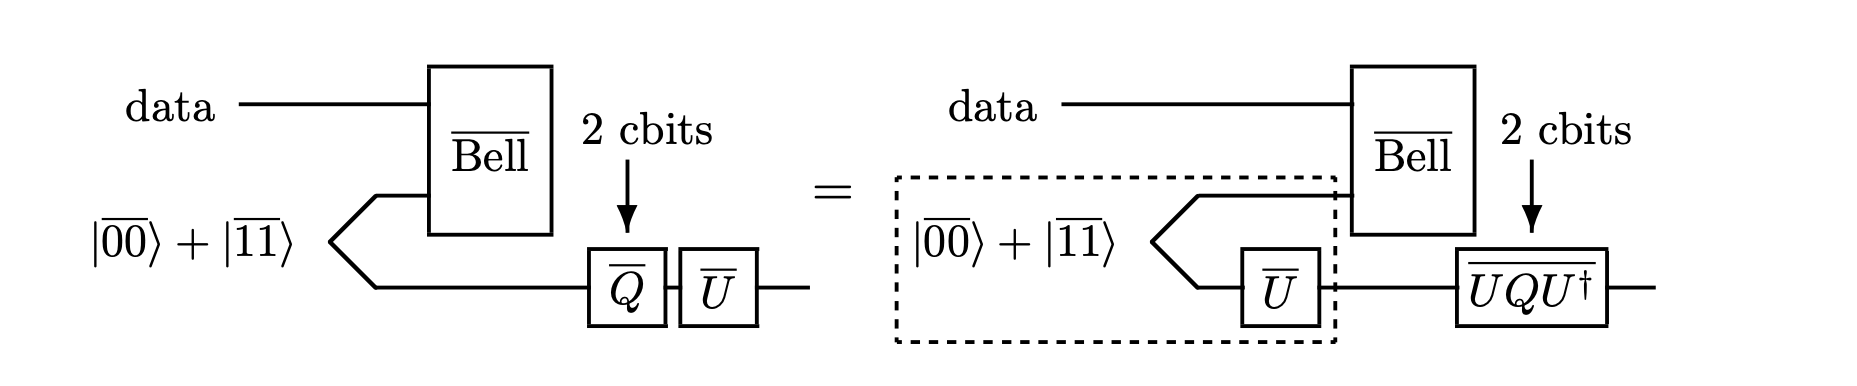
\includegraphics[width=\textwidth]{Mainmatter/images/teleportation_fault.png}
    \caption{Gate teleportation of $\Bar{U}$. The process of teleporting the state followed by $\Bar{U}$ is the same as teleporting the state through a special ancilla with an appropriately modified correction operation.}
    \label{fig:fault_teleport}
\end{figure}
Suppose we were to perform quantum teleportation (this means to apply the require pauli $\Bar{Q}$ gates once we get the instructions from classical measurements) and then follow it, somehow, by an implementation of $\Bar{U}$. Thus on input state $\ket{\psi}$, the overall output state would be $U\ket{\psi}$. 
Now imagine that the receiver (Bob), who controls the output block, perform $\Bar{U}$ earlier than intended, before the senders’s (Alice) measurement outcome instructions.
Eventually Alice performs the logical Bell measurement and sends Bob the two classical bits describing the outcome, corresponding to a logical Pauli $\Bar{Q}$.
To complete the teleportation procedure, Bob needs to do something different now, he can't do the same pauli operation as before: first, he must undo the $\bar{U}$ he performed prematurely, then perform $\Bar{Q}$, and then finally redo $\bar{U}$, now in the correct place. That is, he should implement the gate $\Bar{U}Q\Bar{U}^{\dagger}$. This procedure is pictured in figure $\ref{fig:fault_teleport}$. It may not seem like we have gained anything by doing this, but for some special gates $U$, we have. We can imagine the state $(I \otimes \bar{U})(|\overline{00}\rangle+|\overline{11}\rangle)$ as a special ancilla state, a replacement for the EPR pair normally used in teleportation, and we can prepare it separately. Since it is a fixed ancilla state, independent of the data, we can apply some special tricks to preparing it.

We still have to perform the gate $\Bar{U} \Bar{Q}\Bar{U^{\dagger}}$, which cannot be done ahead of time on the ancilla, since $Q$ depends on the outcome of a logical Bell measurement on the data block. However, the gate $\Bar{U} \Bar{Q}\Bar{U^{\dagger}}$ might be simpler to perform than $\bar{U}$ was. For instance, when $U \in \mathbf{C}_{1}, \bar{U} \bar{Q} \bar{U}^{\dagger} \in \mathcal{P}_{1}$ that is the defining property of the Clifford group. For some gates $U \notin \mathcal{C}_{1}$, it is nonetheless still true that $\bar{U} \bar{Q} \bar{U}^{\dagger} \in \mathbf{C}_{1}$ for any $\bar{Q} \in \mathcal{P}_{1}$. For instance, the $\pi/8$ rotation $R_{\pi/8}$ has this property:
$$
\begin{array}{l}
R_{\pi / 8} X R_{\pi / 8}^{\dagger}=\left(\begin{array}{cc}
0 & e^{-i \pi / 4} \\
e^{i \pi / 4} & 0
\end{array}\right)=e^{i \pi / 4} X P^{\dagger} \\
R_{\pi / 8} Z R_{\pi / 8}^{\dagger}=Z
\end{array}
$$
We sometimes call the set of unitary operators with this property, of conjugating Pauli operators into Clifford group operators, $C_{3} . C_{1}$ is the Pauli group $\mathcal{P}_{n}$, and $C_{2}$ is the Clifford group $\mathcal{C}_{1} .$
One can define a set $C_{k}=\left\{U \mid U Q U^{\dagger} \in C_{k-1} \forall Q \in C_{1}\right\}$, and the teleportation construction tells us how, given appropriate ancilla states, to perform a gate from $C_{k}$ once we know how to perform gates from $C_{k-1}$.

This whole procedure gives us an indication of how to perform a universal set of fault-tolerant gates. For the 7-qubit code, and some similar CSS codes, we already know how to perform all logical Clifford group operations. The Bell measurement is a Clifford group operation, and now we have seen that $R_{\pi / 8} Q R_{\pi / 8}^{\dagger}$ is also a Clifford group operation for $Q \in \mathcal{P}$.  


The correction required after teleportation is a Clifford group gate, for which we already know a fault-tolerant procedure. This yield to the possibility to have universal quantum computation procedure in a complete fault-tolerant way.





\section{Threshold theorem}



The threshold theorem is one of the most remarkable results in fault-tolerant computation. It says that if the error rate of a physical system is below some threshold value, arbitrarily long reliable fault-tolerant quantum computation is possible.




One possible way to prove the threshold theorem and build a reliable quantum computation is by using fault tolerant protocols and concatenating codes.
If an error occurs during a logical gate operation, then Fault-tolerance ensures this error will only propagate to at most one error in each encoded block, after which a cycle of error correction will remove the error. Hence if the failure probability of un-encoded qubits per time step is $p$, then a single level of error correction will ensure that the logical step fails only when two (or more) errors occur. Hence the failure rate of each logical operation, to leading order, is now $p_L = cp^2$, where $p_L$ is the failure rate (per logical gate operation) of a first level logical qubit, and $c$ is the upper bound for the number of possible 2-error combinations which can occur at a physical level within the circuit\footnote{In this specific case $c$ is the number of possible 2-error combinations, because we used a QECC that can correct 1 error. If we use different QECC codes that corrects t-errors the upper bound $c$ becomes: $c=\left(\begin{array}{c}
       G\\
       t+1
 \end{array}\right)$ where G is the total number of gates. 
 
 
 In addition, the logical step fails only when $t+1$ (or more) errors occur. Hence, the failure rate of each logical operation gate, to leading order, is $p_k = cp^{(t+1)}$
 
 
 }.
Hence, thanks to fault tolerance protocols we can decrease the error rate from $p \to cp^2$. 
% If an error occurs during a logical gate operation, then fault-tolerance ensures this error will only propagate to at most $t$ correctable error (depending on which QECC we use) in each encoded block, after which a cycle of error correction that correct $t$ errors will remove them. If the failure probability of un-encoded qubits per time step is $p$, then a single concatenation level of error correction will ensure that the logical step fails only when $t+1$ (or more) errors occur. Hence, the failure rate of each logical operation gate, to leading order, is now $p_k = cp^{(t+1)}$.
% $p_k$ is the failure rate (per logical gate operation) of a first level logical qubit, and $c=\left(\begin{array}{c}
%       G\\
%       t+1
% \end{array}\right)$ where G is the total number of gates. This coefficient is the upper bound for the number of possible ($t+1$)-error combinations if we use a $t$-error correction code, which can occur at a physical level within the circuit.


% For the sake of clarity, in the following lines we suppose that we use a QECC that corrects 1 error. 
% Hence, thanks to fault tolerance protocols we can decrease the error rate from $p \to cp^2$. 
Then, we can reduce the effective error rate achieved even more by concatenation of codes. 
This idea replaces each physical qubit at layer $k$ by an encoded qubit. An example of concatenation using the bit-flip code is shown in figure \ref{fig:codeconc} \footnote{Of course the bit-flip code is insufficient in general since it doesn’t correct phase errors. However, everything we shall demonstrate with the bit-flip code also holds for more general quantum codes, as the 7 qubit code.}.
\begin{figure}[h!]
    \centering
    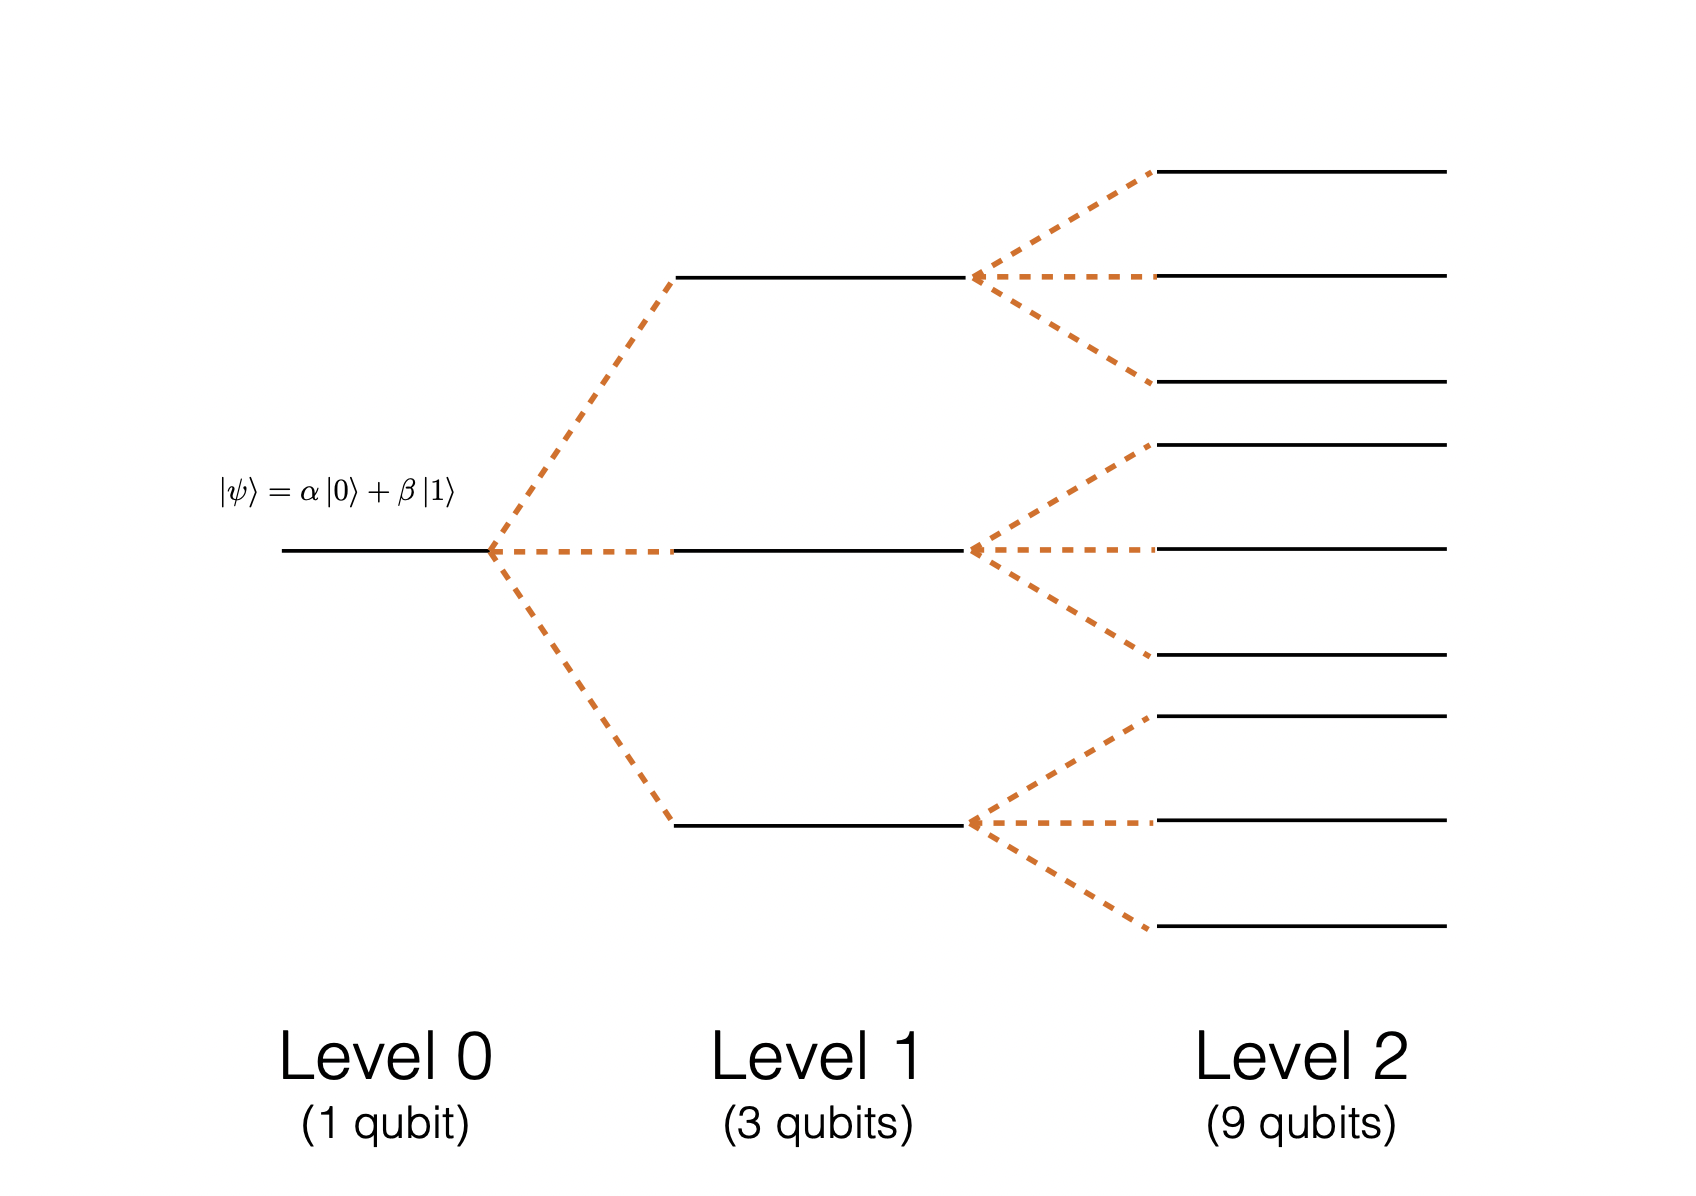
\includegraphics[scale=0.5]{Mainmatter/images/concatenation.png}
    \caption{An illustration of concatenation of the bit flip code. Each qubit at level $k$ is encoded into three qubits at level $k + 1$.}
    \label{fig:codeconc}
\end{figure}

If we perform error correction at each layer of concatenation, then if the bare qubit experiences an error probability of $p$, then after one layer of error correction the logical error probability is $c p^{2}$, and after two layers, the logical error probability is $c\left(c p^{2}\right)^{2}$ (since two blocks have to fail and each block has failure probability $\left.c p^{2}\right)$. With each concatenation later, even though the number of qubits is grows exponentially in k, we get a gain in error probability. That is:
$$
\begin{array}{cccccccccc}
\text { level } 0 & & \text { level } 1 & & \text { level } 2 & & \ldots  & & \text { level } k\\
p &\rightarrow & c p^{2} &\rightarrow & c\left(c p^{2}\right)^{2} &\rightarrow& \ldots &\rightarrow& c^{-1}(c p)^{2^{k}}
\end{array}
$$
And we are guaranteed that this is a gain $(i . e .$, that the error probability decreases with level of concatenation) if
\begin{equation}
p > c p^2
\label{eq:plesscpp}
\end{equation}

Now let us look at the cost of doing this concatenated coding. If the size of the original (unencoded) circuit we want to execute has T gates, and the cost of implementing each gate at the logical level (this depends on the code being used) is at most N physical gates, then the number of gates needed at level 1 of concatenation is at most NT. And for each level of increasing concatenation we must use N times as many gates:
$$
\begin{array}{cccccccccc}
\text { level } 0 & & \text { level } 1 & & \text { level } 2 & & \ldots  & & \text { level } k\\
T &\rightarrow & NT &\rightarrow & N^2T & \rightarrow & \ldots &\rightarrow& N^kT
\end{array}
$$


Note that the number of gates needed grows exponentially in k, but recall that the error probability reduced doubly exponentially in k. This suggests that we can win with this approach. But to see this convincingly, let us see how many gates we need to achieve a given error probability in the computation. Suppose we wish to achieve a final accuracy of $\epsilon \geq 0$ in our simulation of our algorithm.
Then we want that the total error rate is below $\epsilon$: 
$$
T p_{k}=T c^{-1}(c p)^{2^{k}}<\epsilon
$$
for some concatenation level $k$. Here $T$ is the number of logical quantum gates needed to perform the computation (which is the same as the number of gates necessary at the unencoded level), and $p_{k}$ is the error probability per logical gate at concatenation level $k$.


We can solve for $k$ to get
$$
\begin{aligned}
&(c p)^{2^{k}}<\frac{\epsilon c}{T} \\
\Rightarrow \quad & 2^{k}<\log _{c p}\left(\frac{\epsilon c}{T}\right)=\frac{\log_2 \left(\frac{\epsilon c}{T}\right)}{\log_2 (c p)} \\
\Rightarrow \quad & k<\log_2 \left[\frac{\log_2 \left(\frac{\epsilon c}{T}\right)}{\log_2 (c p)}\right]
\end{aligned}
$$
From this upper bound on the concatenation level we can also form an upper bound the number of physical gates we will need to achieve this level $\epsilon$ of logical error. 

We calculated above that at concatenation level $k$ we need $N^{k} T$ gates. Then,
$$
N^{k} T<N^{\log \left(\frac{\log \left(\frac{\epsilon c}{T}\right)}{\log (c p)}\right)} R
$$


But using $\log _{a} x=\frac{\log _{b} x}{\log _{b} a}$, we simplify
$$
N^{\log (\cdot)}=\left(N^{\log _{N}(\cdot)}\right)^{\frac{1}{\log _{N} 2}}=(\cdot)^{\log N}
$$
Using this, the number of gates needed is upper bounded by
$$
\# \text{gates} = T\left(\frac{\log \left(\frac{T}{\epsilon c}\right)}{\log \left(\frac{1}{c p}\right)}\right)^{\log N} \sim  O(T\operatorname{poly}(\log T / \epsilon))
$$
The original $T$ gates are scaled by the factor in braces. This factor is a polynomial in the log (is polylog) in $\frac{1}{\epsilon}$ (inverse error) and in $T$ (the number of gates in the unencoded computation). Therefore the cost of achieving arbitrary error by concatenation scales very favorably, and this is the power of the fault tolerance theorem: we can achieve an arbitrary error probability $\epsilon$ with resources that scale only polylogarithmically in the inverse of the desired error and the complexity of the computation to be performed $(T)$.

Now, let us go back to Eq. \ref{eq:plesscp}, which defines the crucial condition for concatenation to be effective: $p>c p^{2}$. We can compute the value of $p$ that is at the boundary defined by this condition, $p=c p^{2}$. This value of $p$ is called the threshold probability, and is easily seen to be
$$
p_{\mathrm{th}}=c^{-1}
$$
because we want that the error probability decreases further the concatenation goes on.
Thus if the physical error probability is below this threshold probability $p<p_{\mathrm{th}}$, then concatenation and error correction is beneficial. Finally, writing the logical error probability at concatenation level $k$ in terms of $p_{\mathrm{th}}$ gives us
$$
p_{k}=c^{-1}(c p)^{2^{k}}=p_{\mathrm{th}}\left(\frac{p}{p_{\mathrm{th}}}\right)^{2^{k}}
$$

%%%%%%%%%%%
%Da fare
%%%%%%%%%%%
% The behavior of this quantity as a function of $p$, for a fixed $p_{\mathrm{th}}$ and $k$. You will see that if $p$ is a little below the threshold probability the logical error probability quickly goes to zero. In contrast, if $p$ is a little above the threshold probability the logical error probability goes up very quickly. Thus, $p_{\mathrm{th}}$ defines a sharp boundary that specifies when reliable computation is possible and when it is not.


So what is the value of $p_{th}$? This depends heavily on the type of error correction code used, because $c$ depends on the the type of constructions used for gates, measurements, state preparation, etc. Nevertheless, a rough estimate for the threshold probability for the Steane code is given in \cite{Chuang} and the threshold is $p_{th} \approx 10^{-4}$. Thus, if we can get the error rate per gate below this value we can do arbitrary long reliably quantum computation. So if quantum computing architectures can get their fundamental errors (in gates, measurements, state preparation, and idle periods) down to this level, then theory comes in and we are in a safe space to compute.

A more detailed derivation of the threshold theorem can be found in \cite{DanielGottesman}








% This construction can be can be used to reduce the effective error rate achieved by the computation even further. This idea replaces each physical qubit at layer k by an encoded qubit. So the circuit is built by constructing a hierarchy of quantum circuits $C_0$ (the original circuit we wish to simulate), $C1$, $C2$, . . .
% Then if we perform fault tolerant computation and error correction at each layer of concatenation, then if the bare qubit experiences an error probability of $p$, then after one layer of error correction the logical error probability is $cp^2$. In particular if we implement this procedure more and more we decrease the error probability, for example after two layers, the logical error probability is $c(cp^2)^2$ (since two blocks have to fail and each block has failure probability $cp^2$)
% In the first stage of this construction, each qubit in the original circuit is encoded in a quantum code whose qubits are themselves encoded in a quantum code, whose own qubits are encoded yet again, and so forth ad infinitum, as illustrated:
% What is concatenate code? Imagine to encode one qubit with n physical qubits, and then use fault tolerant protocols for gates. If an error occurs in a gate with probability $p$, the probability to have 2 errors goes with the order of $p^2$. By encoding it the effective error rate goes from $p \to Cp^2$, where C is a constant depending on the number of gates that can go wrong. This is an improvement. Concatenate codes make this error falling down smaller and smaller





\section{Toric code}
An active research field in quantum computing is to find codes that will increase $p_{th}$ to larger values. One of the codes that has had a lot of positive feedback and opens up to a larger class of codes (surface codes) is the Toric code.


%\chapter{Entanglement purification and Quantum error correction}
%\include{Mainmatter/EPP}
\chapter{Conclusions}
\include{Mainmatter/conclusion}
\chapter{Appendix}
\subsection*{Quantum Teleportation}
In the teleportation protocol, the two parties (guess who)  share the entangled Bell State and it is implemented via a CNOT gate between the state to be sent (suppose Alice is sending the state) and the part of entangled Bell state Alice has. The CNOT gate creates another entangled state whose measurement Alice will send to the second party, say it's Bob, to perform the measurements accordingly. So if you assume the state to be sent is 1 qubit state after CNOT you will have a 3 qubit state (as Bell sate is 2 qubit state). Now Alice will measure the middle qubit which will be the part of classical information she will communicate to Bob.

So, you see the controlled-NOT acts as an entangling operator without affecting the first qubit (here $\ket{\psi}$) and changing the entangled Bell state and hence its measurement outcome.
A general description of this cool phenomena is shown in figure: 
\begin{figure}[h!]
    \centering
    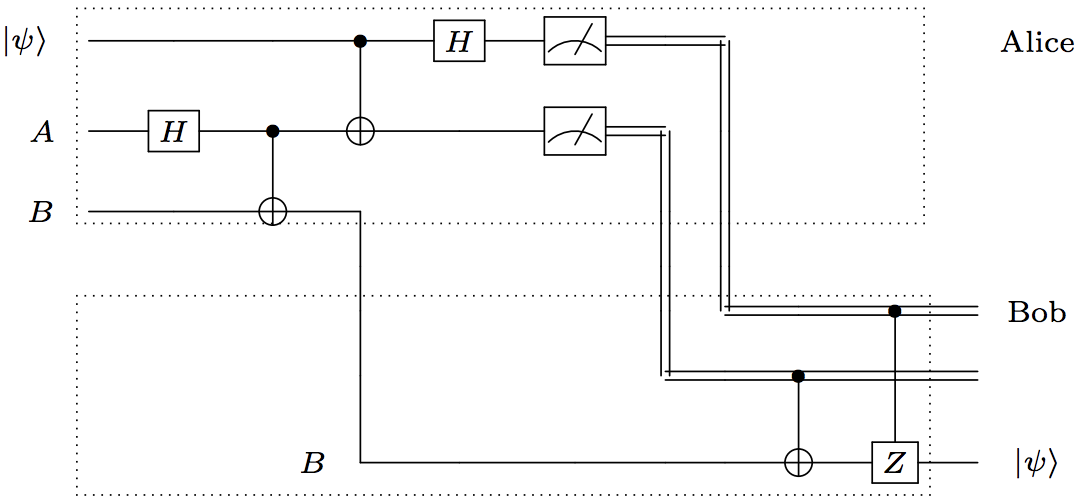
\includegraphics[width=\textwidth]{Mainmatter/images/teleportation-circuit.png}
    \caption{Basic circuit which implements quantum teleportation}
    \label{fig:teleportation}
\end{figure}
Quantum teleportation is very useful in quantum communication because it allows to send classical reliable bits instead of a qubit.
\backmatter
\include{Backmatter/references}
\printbibliography
\nocite{*}
\end{document}

%%%%%%%%%%%%%%%%%%%%%%%%%%%%%%%%%%%%%%%%%%%%%%%%%%%%%%%%%%%%%%%%%%%%%%%%%%%%%%%
%                                                                             %
% *** END OF THIS BACHELOR THESIS PROJECT ***                                 %
%                                                                             %
%%%%%%%%%%%%%%%%%%%%%%%%%%%%%%%%%%%%%%%%%%%%%%%%%%%%%%%%%%%%%%%%%%%%%%%%%%%%%%%